\chapter{Process Mining}
\label{process_mining}

Objective of this chapter is to introduce some basic concepts about \textbf{Process Mining}, starting from Business Process 
Management, defining the concept of Process and finally presenting some tools available on the market. The purpose of this 
first part is to allow also to not expert readers to understand the work done in this thesis.

At a first place there is a little introduction in the world of \textbf{Business Process Management} in section 
\ref{process_mining:bpm} which helps to better understand the utility of process mining.
After that there is a general overview of process mining in section (\ref{process_mining:overview}) where are described some 
key notions of the theme: different kind of process mining, principles and standards.
Section \ref{process_mining:algorithms} focuses on process model discovery, illustrating the most used \textbf{algorithms} in 
this field.
Section \ref{process_mining:tools}, the last of the chapter, has the purpose of show the main software \textbf{tools} used to 
work with process mining.


\section{Business Process Management}
\label{process_mining:bpm}
BPM is the set of all activities to support and improve organisation performance by managing chains of events, tasks, and 
decisions that ultimately add value to the organisation. It includes concepts, methods, and techniques to support the design, 
administration, configuration, enactment, and analysis of business processes \cite{DBLP:books/WeskeBPM}.

A Business Process is described as “a collection of related and structured activities undertaken by one or more organisations 
in order to pursue some particular goal. Within an organisation a business process results in the provisioning of services or 
in the production of goods for internal or external stakeholders. Moreover business processes are often interrelated since 
the execution of a business process often results in the activation of related business processes within the same or other 
organisations” \cite{DBLP:journals/infsof/LindsayDL03}.

Around the notion of business process borns \textbf{Business Process Management}. As described in 
\cite{DBLP:books/sp/DumasRMR18} Business Process Management (BPM) is the set of activities needed to define, optimize, monitor 
and integrate business processes in order to make effective company's business. In \cite{DBLP:books/WeskeBPM} is described the 
BPM \textbf{``lifecyle''} shown in the Figure \ref{images:bpm_lifecycle}.

\begin{figure}[!ht]
    \centering
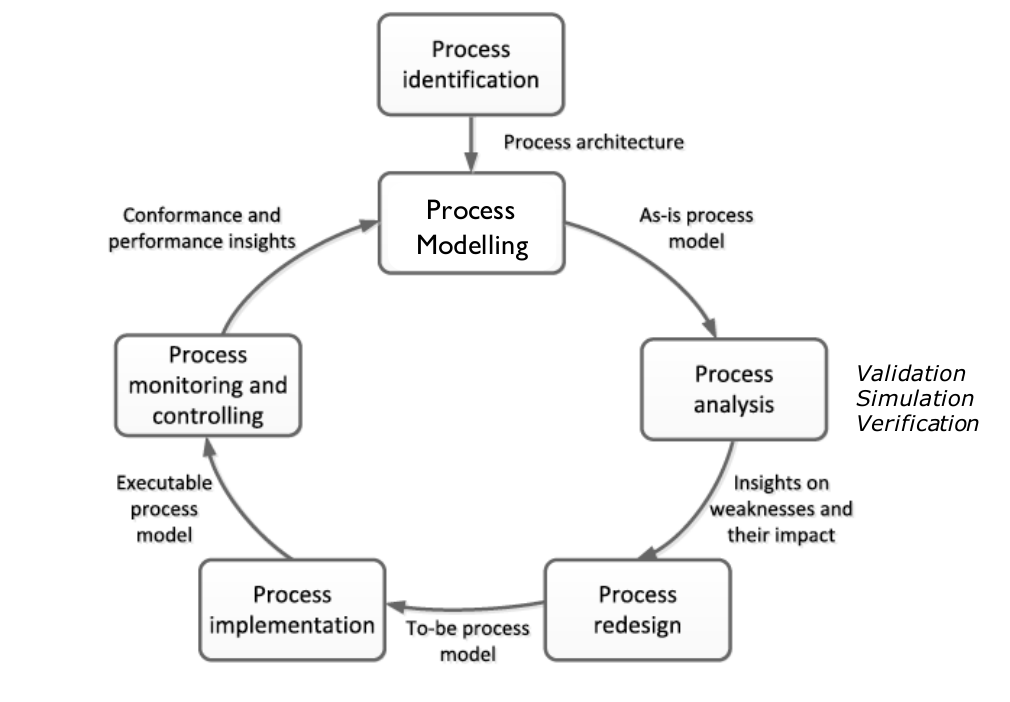
\includegraphics[width=\textwidth]{images/bpm_lifecycle.png}
    \caption{Business Process Management lifecycle \cite{DBLP:books/sp/DumasRMR18}}
    \label{images:bpm_lifecycle}
\end{figure}

We can see that there are 6 phases in the BPM lifecycle and that 5 of them are in a cycle: this means that these can 
be executed many times in order to continually refine the business processes. Let's describe shortly the different 
phasis:

\begin{itemize}
    \item \textbf{Process identification}: this step is executed only one time when the company start to model its 
        processes (for each process that must be deal with).

    \item \textbf{Process modeling}: this stage consists in the building of a process model that describe the real 
        life process. This activity is based on interviews with customer and industry experts and produce a model 
        of how the process is actually performed (as-is process model).

    \item \textbf{Process analysis}: at this level the ``as-is process model" is validated and design issues are
        identificated (this validation has 3 steps: validation, simulation and verification). A the end of this 
        phase there is a report of the model's weaknesses.

    \item \textbf{Process redesign}: if in the previous step some critical weakness were found, in this stage they 
        must be removed building the ``to-be process model".

    \item \textbf{Process implementation}: this phase has the goal of transform the to-be process model in a set 
        of rules that to be applied in order to change the current process execution. This set of rules is called 
        ``executable process model".

    \item \textbf{Process monitoring and controlling}: the last step of the lifecycle is the monitoring of the 
        changes applied to the process: in this task metrics are measured to understand how well the process 
        is performing. Is in this phase that process mining comes in to help to understand if there are some 
        problems and to improve process performance.
    
\end{itemize}


\section{Business Process Modelling Language}

The modeling step of the lifecycle needs some language to visualize and compare different process models: there are a lot of 
different notations but the most common is \textbf{Business Process Model and Notation} \cite{DBLP:journals/Chinosi} (BPMN) that is 
establishing itself as a de-facto standard. Another important and very used notation are \textbf{Petri Net}s (PN) 
\cite{PetriNetIntroduction}. They are pretty useful when there are verification needs.


\subsection{BPMN}
It was originally conceived and developed by the Business Process Management Initiative (BPMI). It is currently 
maintained by the Object Management Group (OMG). BPMN provides a notation that is simple and standard to make it 
understandable by people with different education and competence: management personnel, analysts and developers.

It maps 4 different types of objects: 

\begin{itemize}
    \item \textbf{Flow objects}, that can be events, activities or gateways. Events are represented as circle that can 
        contains other symbols to specify the type of the event. They can be Start, Intermediate or End events. Activities 
        are tasks that need to be done (sometimes they can be subprocess). Gateways determine the flow of the process and 
        in general are used to split and join different process behaviours.
    \item \textbf{Connecting Objects}, that can be sequence that allows to build the process flow, message that are used to 
        show the exchange of messages between different actors, or association that is used to associate Artifact, data or 
        text to a Flow Object. 
    \item \textbf{Swimlanes}, pools or lanes, used to organize different acitvities and in general lanes are sub-part of pools
    \item \textbf{Artifacts}, files, documents, objects, annotations, and so on.
\end{itemize}

For this thesis work only simple and basic Flow objects have been used, those shown in figure \ref{images:bpmn_flow_obj}.

\begin{figure}[!ht]
    \centering
    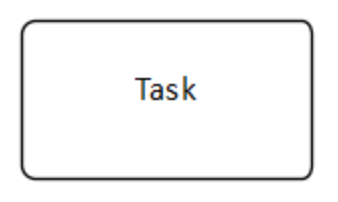
\includegraphics[width=30mm]{images/bpmn_task.png}
    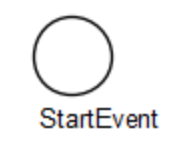
\includegraphics[width=20mm]{images/bpmn_start_event.png}
    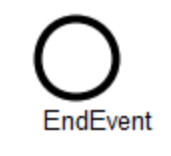
\includegraphics[width=18mm]{images/bpmn_end_event.png}
    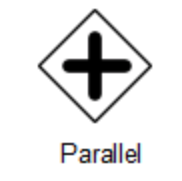
\includegraphics[width=16mm]{images/bpmn_parallel.png}
    
\includegraphics[width=18mm]{images/bpmn_exclusive.png}
    \caption{BPMN flow objects used in the thesis}
    \label{images:bpmn_flow_obj}
\end{figure}


\begin{figure}[!ht]
    \centering
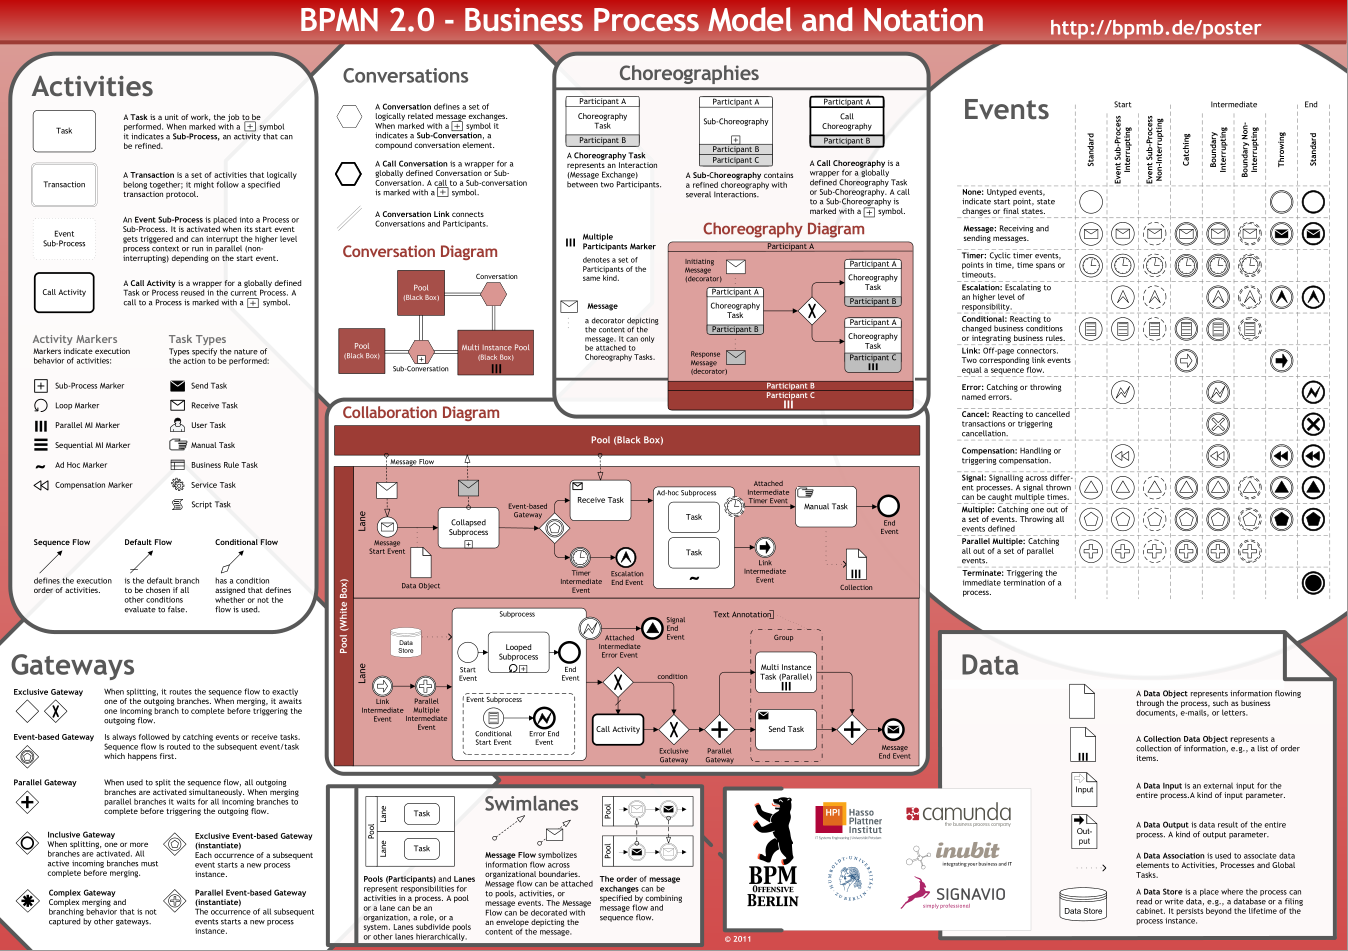
\includegraphics[width=\textwidth]{images/bpmn_manifesto.png}
    \caption{BPMN Manifesto}
    \label{images:bpmn_manifesto}
\end{figure}

BPMN allows the representation of interprocess communication or also process that include two or more stakeholders, it can 
be used for exceptions handling and other complex situations. For a complete set of BPMN elements see the Figure 
\ref{images:bpmn_manifesto}


\subsection{Petri Net}
Petri Nets are a really powerfull notation largely used in theoretical computer science in a big number of fields. They were 
formalized by Carl Adam Petri in its PhD thesis. They allow to model statics and dynamics systems throught a set of places, 
a set of transitions (or events) and a set of arcs that join places and transitions (Figure \ref{images:petri_net_elements} 
shows the representations of these elements). There are few and simple elements that allow for a huge power and flexibility. 
Dynamic systems can be described through the use of tokens that assumes different meanings based on the context: in BPM they 
are instances of the process. Tokens cross the net based to the ``fire rule": in practice a transiton can be crossed only if 
all its input places have the necessary number of tokens and in this case it generates the needed number of tokens for each 
of its output places.

\begin{figure}[!ht]
    \centering
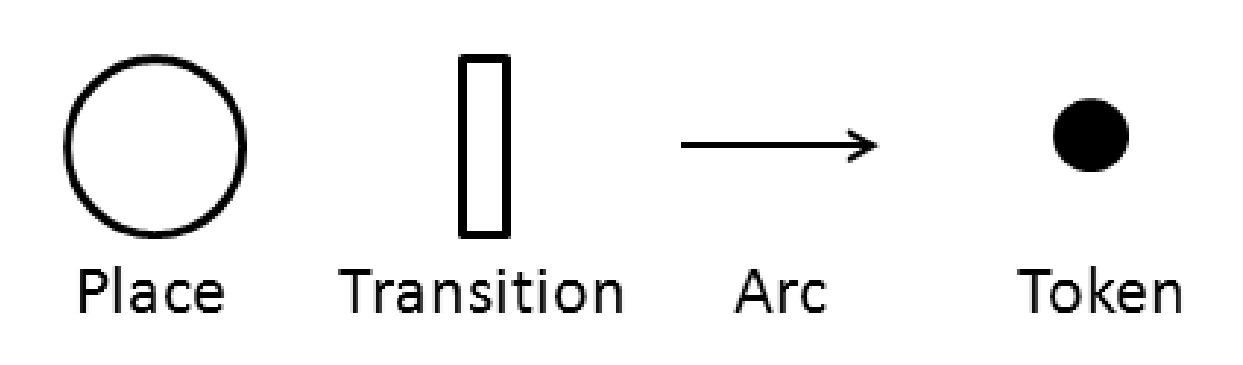
\includegraphics[width=70mm]{images/petri_net_elements.jpg}
    \caption{Petri net elements}
    \label{images:petri_net_elements}
\end{figure}

\section{Overview on Proess Mining Techniques}
\label{process_mining:overview}
The basic idea of the process mining is to infer, monitor and improve real life processes getting knowledge from 
software tool's logs.
Process mining includes the discovery of a process model (an automatic modeling) starting from the logs, the 
conformance checking between a logs and their discovered model, the individuation of relationship between people 
and the prediction of what will happens in a specific instance of a process.
process mining can be considered as a field that cross through Business Intelligence, Data Mining and Business 
Process Management.

\begin{figure}[!ht]
    \centering
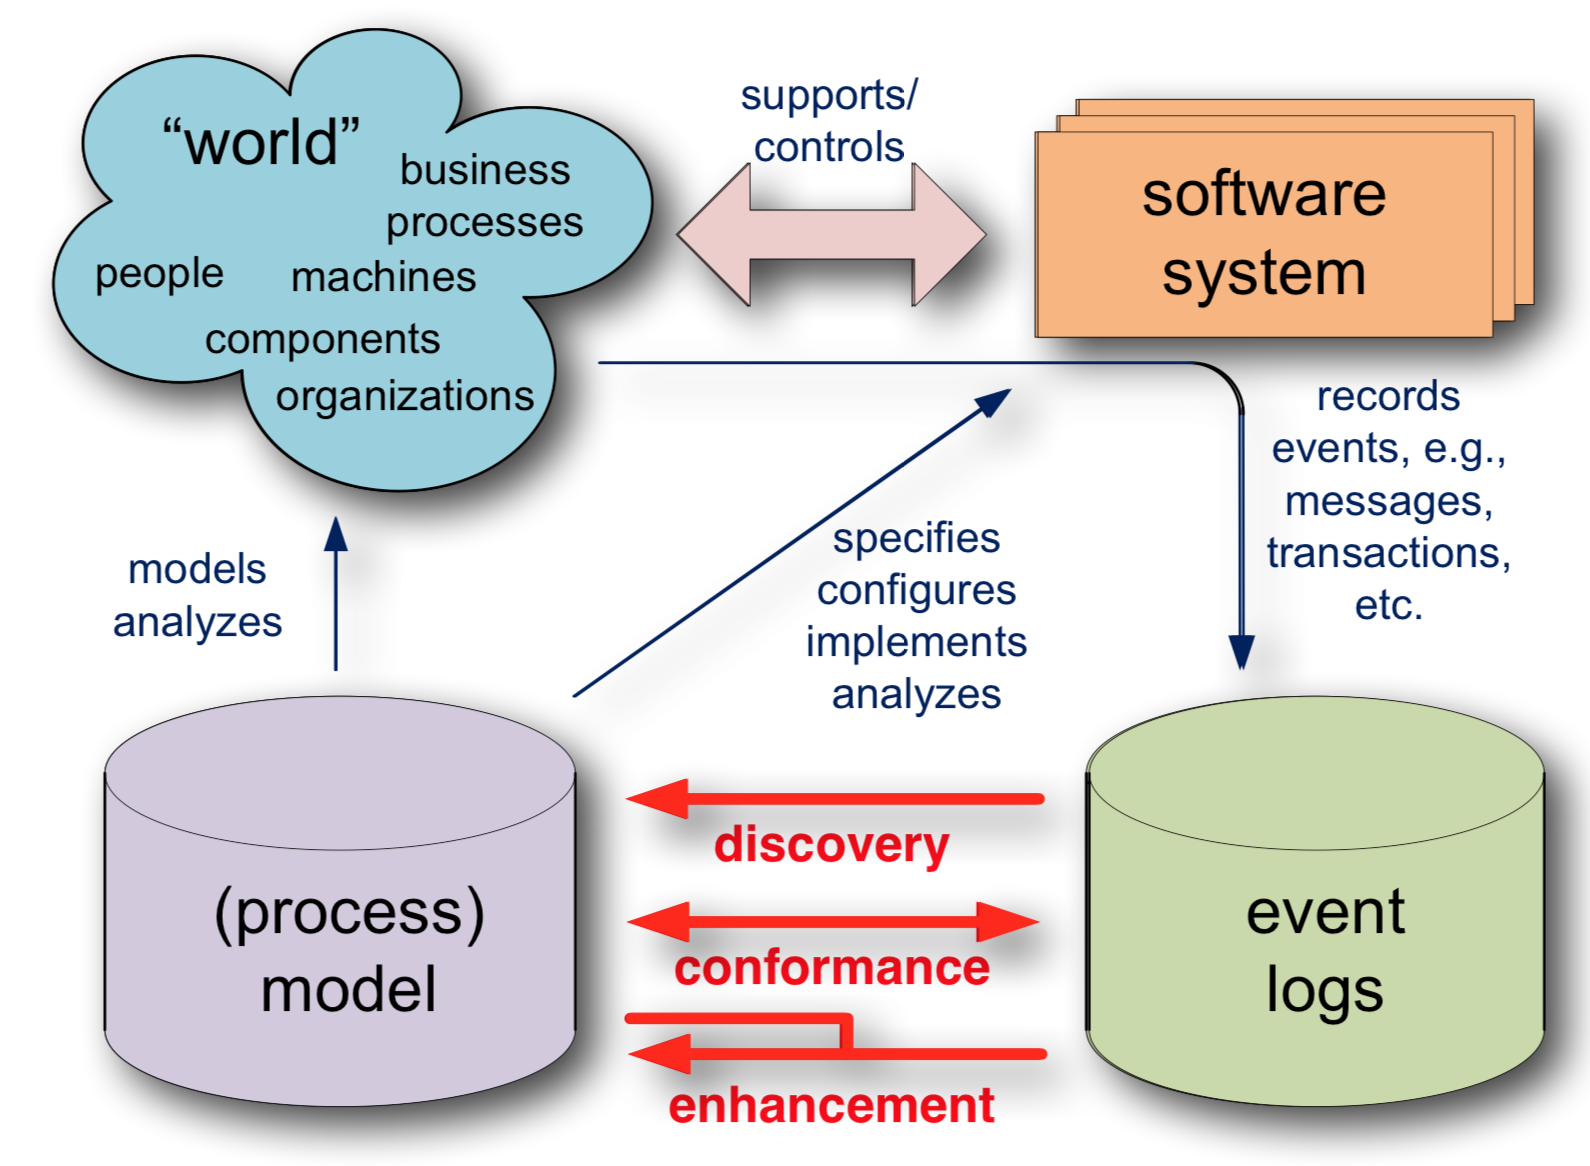
\includegraphics[width=\textwidth]{images/pm_resume.png}
    \caption{Schematic representation of process mining \cite{DBLP:conf/bpm/ProcessMiningManifesto}}
    \label{images:pm_resume}
\end{figure}

There are three forms of process mining:

\begin{itemize}

    \item \textbf{Process discovery}: these techniques allow to process a log, extract information from it and build a 
        process model with these information.

    \item \textbf{Conformance checking}: this type of process mining has the goal of evaluate the quality of a model: to 
        do so it compare the model with a log of the same process and measure how well they conform each other.

    \item \textbf{Enhancement}: in this case the idea is to extend or improve an existing process model using information 
        recorded on some event log.
    
\end{itemize}

\begin{figure}[!ht]
    \centering
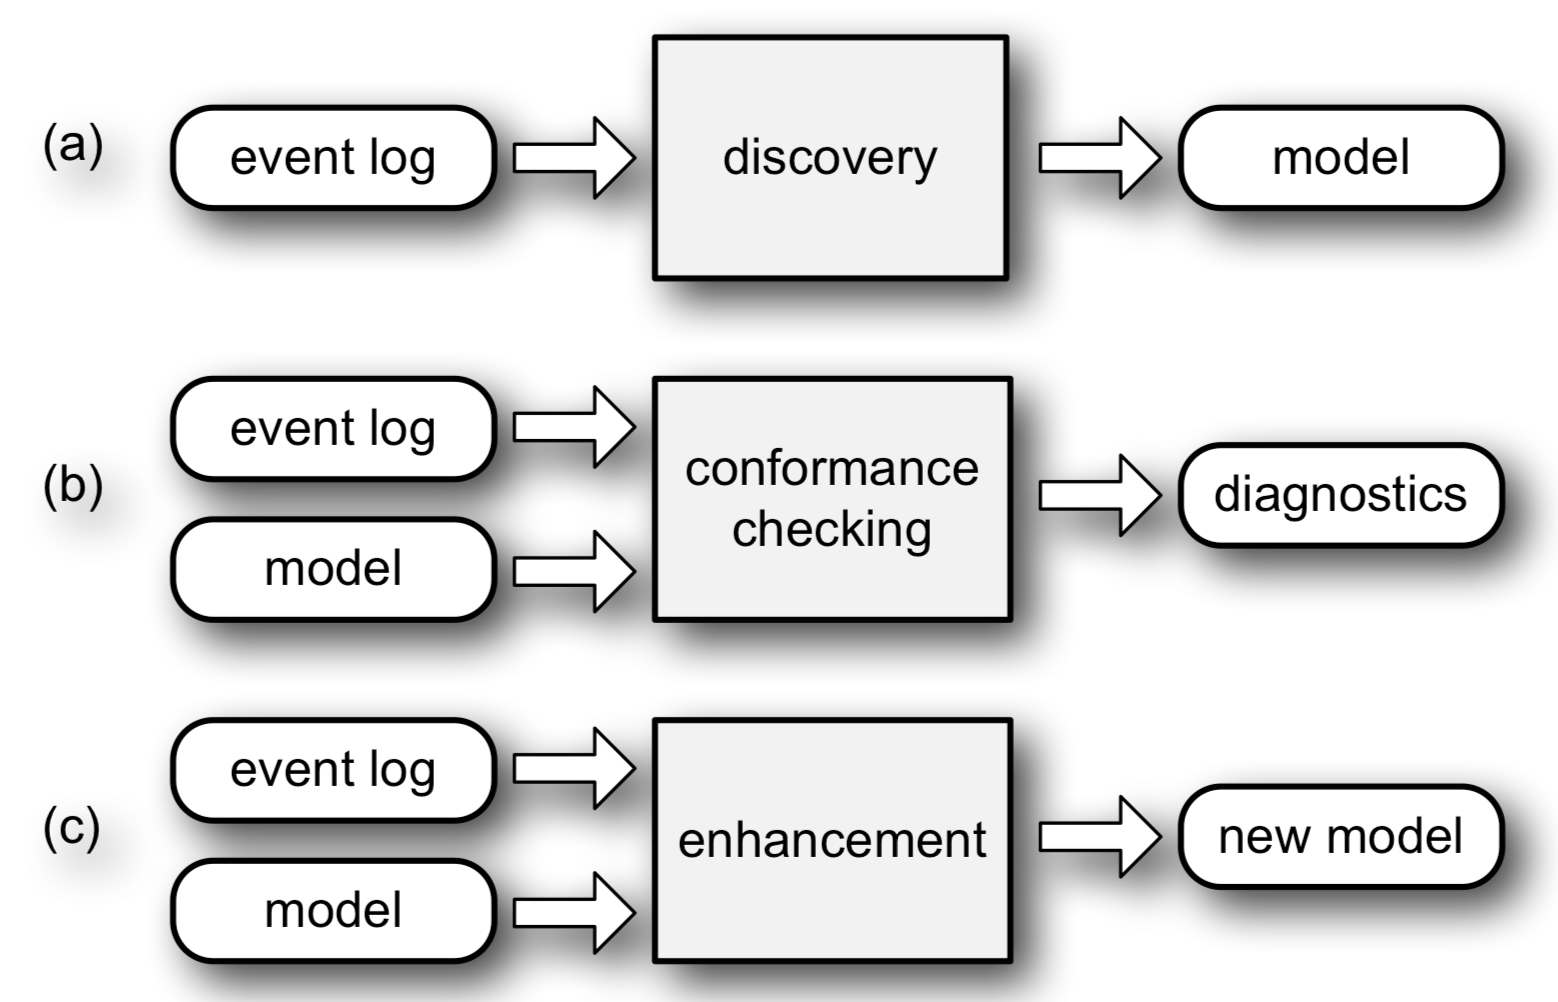
\includegraphics[width=\textwidth]{images/pm_io.png}
    \caption{Different process mining types input/output \cite{DBLP:conf/bpm/ProcessMiningManifesto}}
    \label{images:pm_io}
\end{figure}

It is important to specify that process mining is not limited to offline analysis even if is based on historical event data, 
infact it can be used even for running cases. For example it can be used to predict the completion time of a process instance 
or the choices a user will take in certain conditions, etc.

Process mining is a valuable methodology for most of the phases shown in Figure \ref{images:bpm_lifecycle}.

In Figure \ref{images:pm_project} are shown all steps of a process mining project.
First of all there is a planning activity and a justification for this planning. The second step consist in the extraction 
of all the interisting information needed in the project, current data available, and a good understanding of the domain. 
The result of this activity is a set of artifacts such as historical data, handmade models and objectives.
The next stage is the building of a control-flow model through the use of automated process discovery techniques.
In step 3 control-flow model is extended with other perspectives (documents, time, and resources). The last stage is the 
use of the models created in previous steps for operational support (intervene, predict, and recommend running processes).
Last stages can only be reached if the process is sufficiently stable and structured.

\begin{figure}[!ht]
    \centering
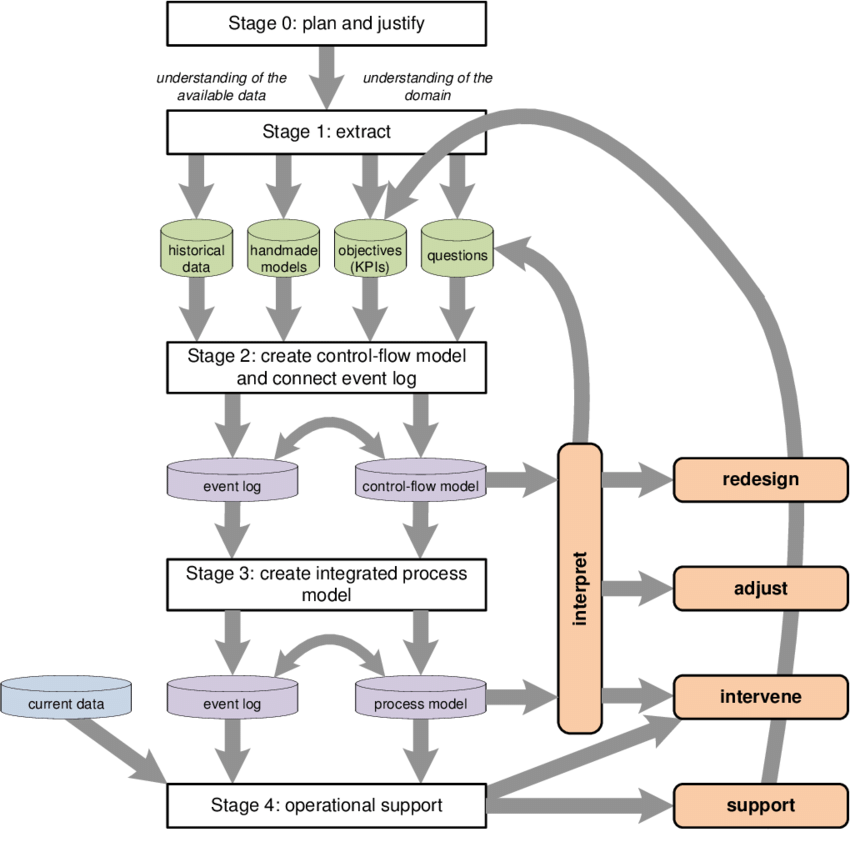
\includegraphics[width=\textwidth]{images/pm_project.png}
    \caption{Steps in a process mining project \cite{DBLP:conf/bpm/ProcessMiningManifesto}}
    \label{images:pm_project}
\end{figure}

As seen before logs are a central concept in process mining but until now the quality of the logs have not been considered 
even if the value of the results of a process mining activity mostly depends by the input. This means that with a poor or not 
precise log we will have not good results.
In Process Mining Manifesto there are a classification of the log value in 5 levels shown in Figure \ref{images:pm_loglevels}.

\begin{figure}[!ht]
    \centering
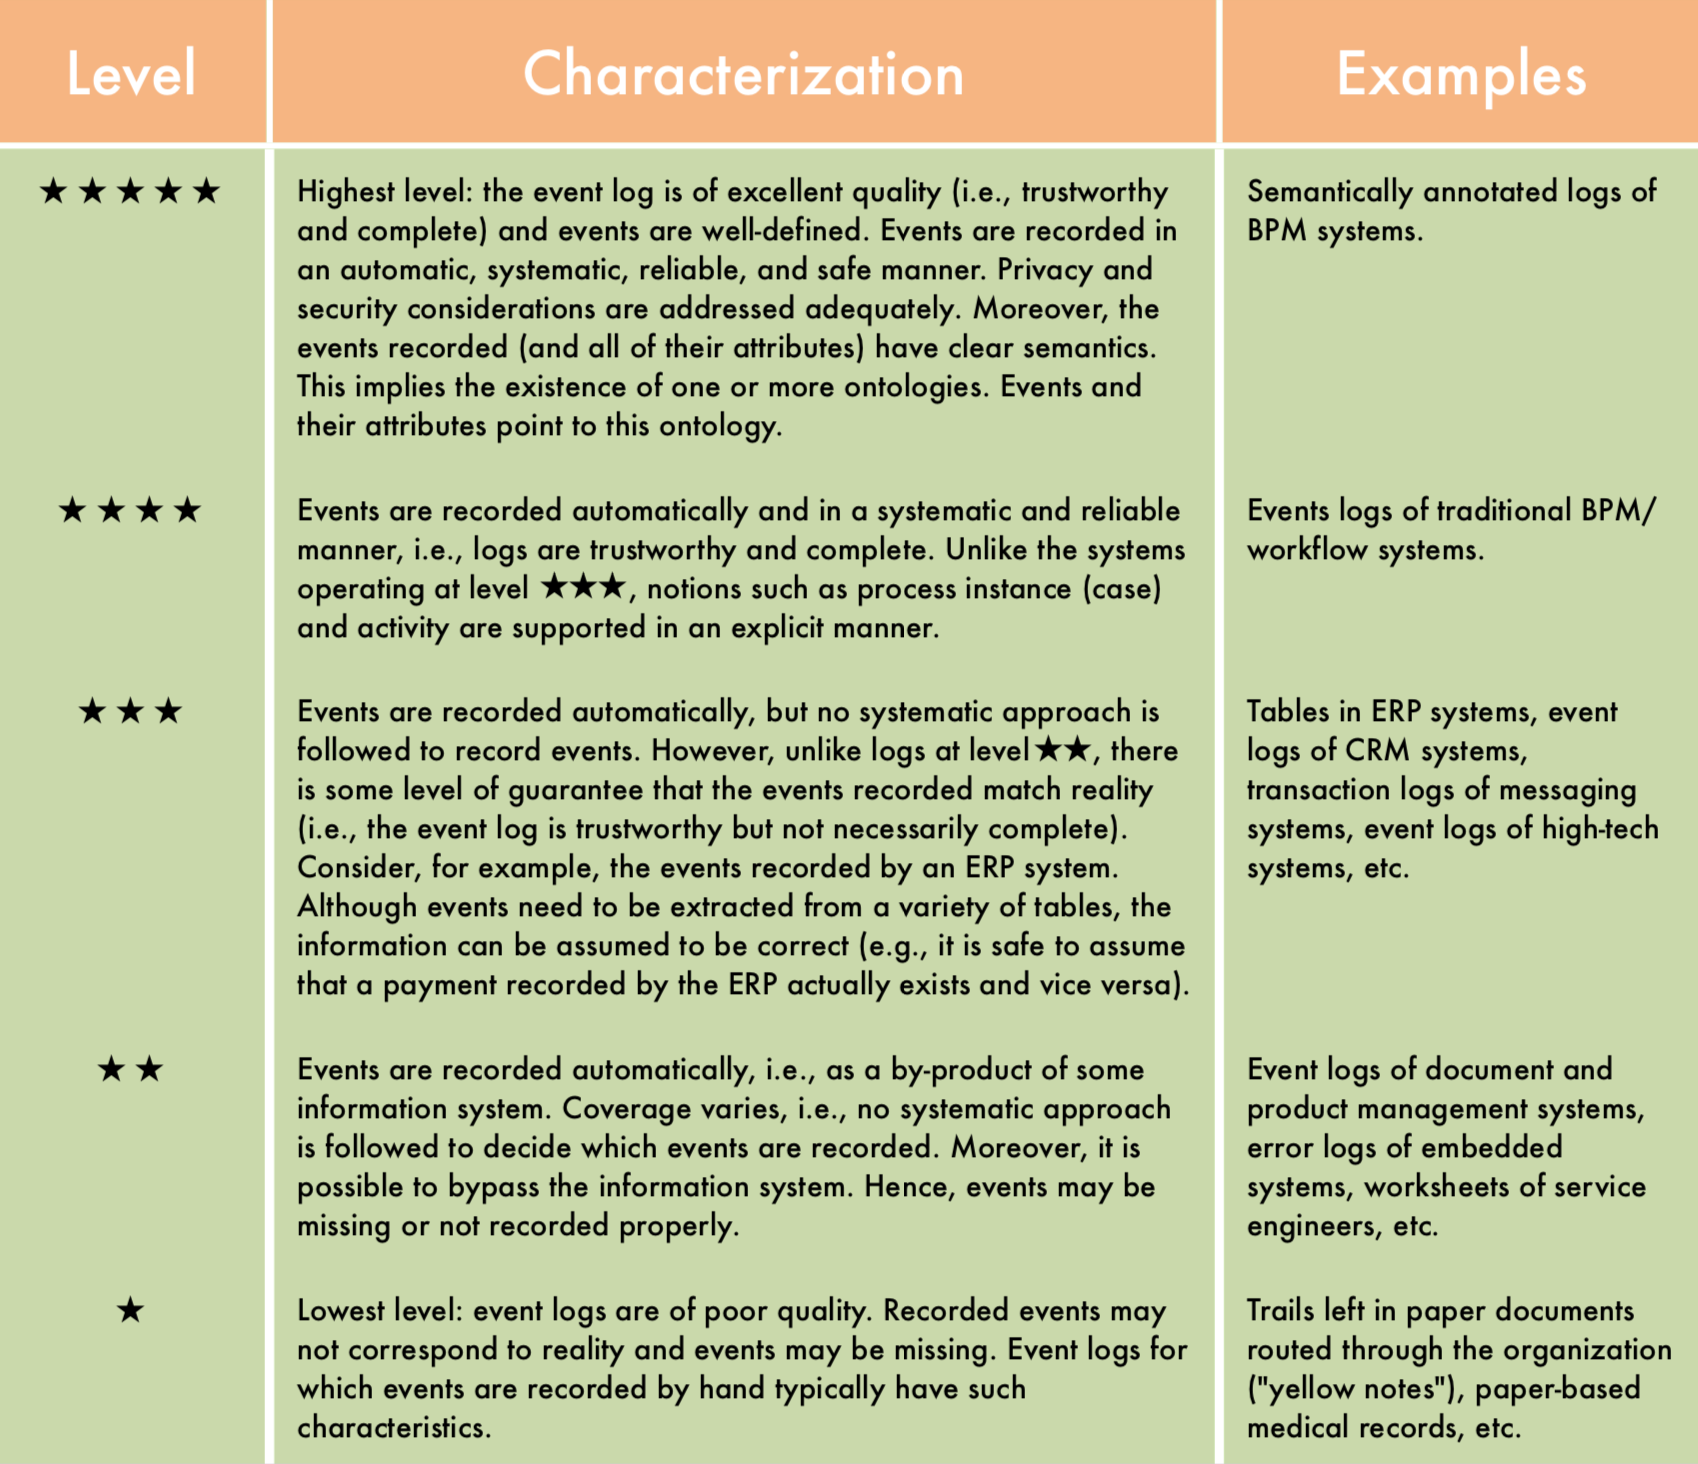
\includegraphics[width=\textwidth]{images/pm_loglevels.png}
    \caption{Maturity levels for event logs \cite{DBLP:conf/bpm/ProcessMiningManifesto}}
    \label{images:pm_loglevels}
\end{figure}

The last important thing to explain about logs is how they are formalized: in the available tools different formats are 
supported (csv, xls, etc.) but in the years a specific format for event logs was developed. \textbf{XES} (Extensible Event 
Stream) is an XML-based standard with the purpose to provide a generally-acknowledged format for the interchange of event 
log data between tools and application domains \cite{XESstandard}.
When designing the XES standard, the following goals have been used as guiding principles:
\begin{itemize}
    \item \textbf{Simplicity}, XES logs should be easy to parse and to generate, and they should be equally well 
        human-readable.
    \item \textbf{Flexibility}, the XES standard should be able to capture event logs from any background, no matter what 
        the application domain or IT support of the observed process. 
    \item \textbf{Extensibility}, it must be easy to add new constructs to the standard in the future while maintaining 
        backward and forward compatibility.
    \item \textbf{Expressivity}, all information elements must be strongly typed, and there must be a generic method to 
        attach human-interpretable semantics to them.
\end{itemize}

Example of XES standard in listing \ref{listing:xes}.

\begin{lstlisting} [caption = {Part of a trace in a XES file}, label = {listing:xes}]
<trace>
    <string key="concept:name" value="Case3.0"/>
    <event>
        <string key="concept:name" value="A"/>
        <int key="concept:instance" value = "1"/>
        <string key="org:resource" value="UNDEFINED"/>
        <date key="time:timestamp" value="2008-12-09"/>
        <string key="lifecycle:transition" value="complete"/>
    </event>
</trace>
\end{lstlisting}


The last important aspect to cover talking about Process Mining is the measure of the results that are being obtained: in this 
context the paper \cite{DBLP:conf/ReplayQualityParameters} introduce four parameters that allow to measure the quality of a discovered 
model in comparison to the event log that generated it: 

\begin{itemize}
    \item \textbf{Fitness}: quantifies the extent to which the discovered model can accurately reproduce the cases recorded 
        in the log.

        \(Fitness = 1 - \frac{\textrm{cost for aligning model and event log}}{\textrm{Minimal cost to align arbitrary event log on model and vice versa}}\)

    \item \textbf{Precision}: this value measures the level of underfitting, i.e. a poor precision means that a model admits 
        unusual behaviors than those shown in the logs.

        \(Precision = 1 - \frac
            {\sum_{\textrm{visited markings}} \#visits * \frac{\textrm{\#outgoing edges} - \textrm{\#used edges}}{\textrm{\#outgoing edges}}}
            {\textrm{\#total marking visits over all markings}
        }\)
        
    \item \textbf{Generalization}: is a measure of the model overfitting: an high level of generalization means that the model 
        can handle behaviors not seen in the log, maybe because not yet observed.

        \(Generalization = 1 - \frac
        {\sum_{\textrm{nodes}} \sqrt{\#executions}^{-1}}
        {\textrm{\#nodes in tree}}
        \)
        
    \item \textbf{Simplicity}: this param try to define a level of human readability of the process model.
    
        \(Simplicity = 1 - \frac{\textrm{\#duplicate activities} + \textrm{\#missing activities}}{\textrm{\#nodes in process tree} + \textrm{\#event classes in event log}}\)
        
\end{itemize}

\begin{figure}[!ht]
    \centering
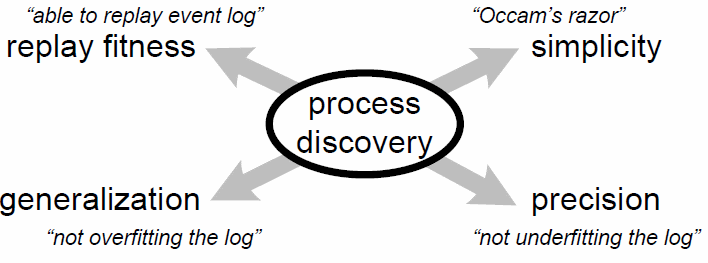
\includegraphics[width=80mm]{images/model_quality.png}
    \caption{Fitness, precision, generalization and simplicity \cite{DBLP:conf/ReplayQualityParameters}}
    \label{images:model_quality}
\end{figure}

Fitness, precision and generalization are measured replaying the traces in the original event log on the discovered process 
model with the format of Petri Net. This is a simple but, potentially, very long task and if done manually is very error prone. 


\section{Discovery algorithms}
\label{process_mining:algorithms}
This section start to focus on the discovery branch of process mining. In order to infer a model from an event log 
we can choose between different algorithms; there is not the best algorithm or the worst but for each case there is an 
algorithm that fits better the environment.

\subsection{Overview of the Alghoritms}

Here is a list of the most used algorithms: 

\begin{itemize}
    \item \textbf{Alpha Miner} 
    is one of the most precise algorithms. It builds a Petri Net generating a table of relationship between all events 
    (causality, parallel or nothing). It is very used in literature beacuse it is relatively simple to implement but it has 
    some known limitations: for example it cannot model loops of length 1 or 2. In order to remove this gap there are two 
    versions of the algorithm: rispectively Alpha+ and Alpha++.
    
    \item \textbf{Fodina}
    is a discovery method based on Heuristic Miner but more reliable when the event log is very noisy. Thanks to this 
    capability it can also handle the discovery based on user inputs. Its properties are discussed in \cite{DBLP:journals/dss/Fodina}.
    
    \item \textbf{Inductive Visual Miner} is described in \cite{DBLP:conf/bpm/InductiveVisualMiner}.
    This is more a tool than an algorithm, in fact it builds a chain of tasks and shows the changes live in a visual 
    format. Events can be filtered to hide them from the model, then Inductive Miner is used to discover the process 
    model. Than is possible to highlight important events, enrich the model and finally to animate it; animate a model 
    means to show different instances of the process in action using tokens that pass through different model steps over 
    time.
    
    \item \textbf{ILP Miner} is presented in \cite{DBLP:journals/fuin/ILPMiner}.
    This algorithm is based on Integer Linear Programming (ILP) techniques (also defined Constraint Programming). ILP 
    miner guarantee a fitness of 1, that means, that the model generated includes all the possibile traces found in 
    the log. This can be a wonderfull feature but not always: in most real-life processes there is some noise in the log, 
    some extremly rare events that should be ingored in the model in order to obtain a result closer to the real-life 
    process. Over that the fact that all possible traces are modeled can bring to an highly unreadable petri net 
    because the number of elements can grow a lot.
    Another negative aspect of this algorithm is that its execution time is bigger than others because ILP problems need 
    a lot of calculation to be solved.
    
    \item \textbf{Fuzzy Miner} was introduced in \cite{DBLP:conf/bpm/DiscoFuzzyMiner} and it is the algorithm used in the software tool Disco 
    for the process discovery. The Fuzzy Miner was the first mining algorithm to introduce the “map metaphor” to process mining, 
    including advanced features like seamless process simplification and highlighting of frequent activities and paths. The 
    result is a set of interesting and reliable information easy to understand also domain experts that do not have any 
    experience on process mining.
    
\end{itemize}


\subsection{Best fitting algorithms}
This section introduce three discovery algorithms which are that used in the practical part of the thesis:

\begin{itemize}

    \item \textbf{Heuristic Miner}:
    as alpha miner also heuristic miner mine the control-flow perspective of a process model building a dependency graph 
    but in a different manner: in fact it uses frquences of events to build this table. For example more 
    frequently a task ``A" directly follows another task B, and the less frequently the opposite occurs, the higher the 
    probability that ``A" causally follows ``B". This allow for noise management because rare events connection can be 
    omitted from the model. The usual output of this algorithm is a Heuristic Net or a Petri Net. While Heuristics Miner has 
    been shown to achieve relatively good fitness and precision in the presence of noise, in \cite{DBLP:conf/icdm/SplitMiner} is explained 
    that it still outputs spaghetti-like and unsound process models when applied to large real-life event logs.

    \item \textbf{Inductive Miner}:
    this is one of the fews algorithms that guarantee the soundness of the process model inferred. It uses a divide-and-conquer 
    approach to discover process trees: It first creates a DFG, filters infrequent directly-follows dependencies, and identifies 
    cuts in the filtered DFG. A cut is a control-flow dependency along which the log can be bisected. The identification of cuts 
    is repeated recursively, starting from the most representative one until no more cuts are found. Once all cuts are 
    identified, the log is split into portions (one per pair of consecutive cuts) and a process tree is generated from each 
    portion.
    In order to divide the activities in log L IM searches for a characteristic division of activities into disjoint sets, a cut, 
    of the directly-follows graph. Each operator (×, →, ∧ or cycle) has a characteristic cut of the directly-follows graph. 
    If such a characteristic matches, IM selects the corresponding operator. Otherwise, a flower model, allowing for all 
    sequences of activities, is returned. Than IM recurses until the model is completely discovered.
    

    \item \textbf{Split Miner}: 
    starting from a log, Split Miner produces a BPMN model in five steps as shown in Figure \ref{images:split_miner_steps}.

    \begin{figure}[!ht]
        \centering
    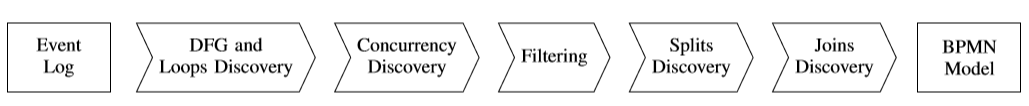
\includegraphics[width=\textwidth]{images/split_miner_steps.png}
        \caption{Split miner steps \cite{DBLP:conf/icdm/SplitMiner}}
        \label{images:split_miner_steps}
    \end{figure}

    Like the Heuristics Miner, the first step is to construct the DFG, but unlike the latter, Split Miner does not immediately 
    filter the DFG. Instead, it analyzes it to detect self-loops and short-loops and to discover concurrency relations 
    between pairs of tasks. Whenever a likely concurrency relation between a and b is discovered, the arcs between these two 
    tasks are pruned from the DFG. The result is called: pruned DFG (PDFG). In the third step, a filtering algorithm is 
    applied on the PDFG to strike balanced fitness and precision maintaining low control-flow complexity. In the fourth step, 
    split gateways are discovered for each task in the filtered PDFG with more than one outgoing arc. This is followed by the 
    discovery of join gateways that is the last step of the alghoritm.
    
\end{itemize}


\section{Tools}
\label{process_mining:tools}

Process mining is a relatively new area of research but it is enough mature to have a set of support tools that enable the 
application of its principles. These software tools implements some of algorithms listed in the previous section, using 
standards and offering a graphical approach.

\subsection{ProM}
ProM is an extensible framework, it is platform independent as it is implemented in Java, and can be downloaded free.
It supports a wide variety of process mining techniques in the form of plug-ins (this is why it is defined as extensible). 
ProM UI is organized in three subsections: \textbf{Object view}, \textbf{Action view} and \textbf{Visualization view}.

\begin{figure}[!ht]
    \centering
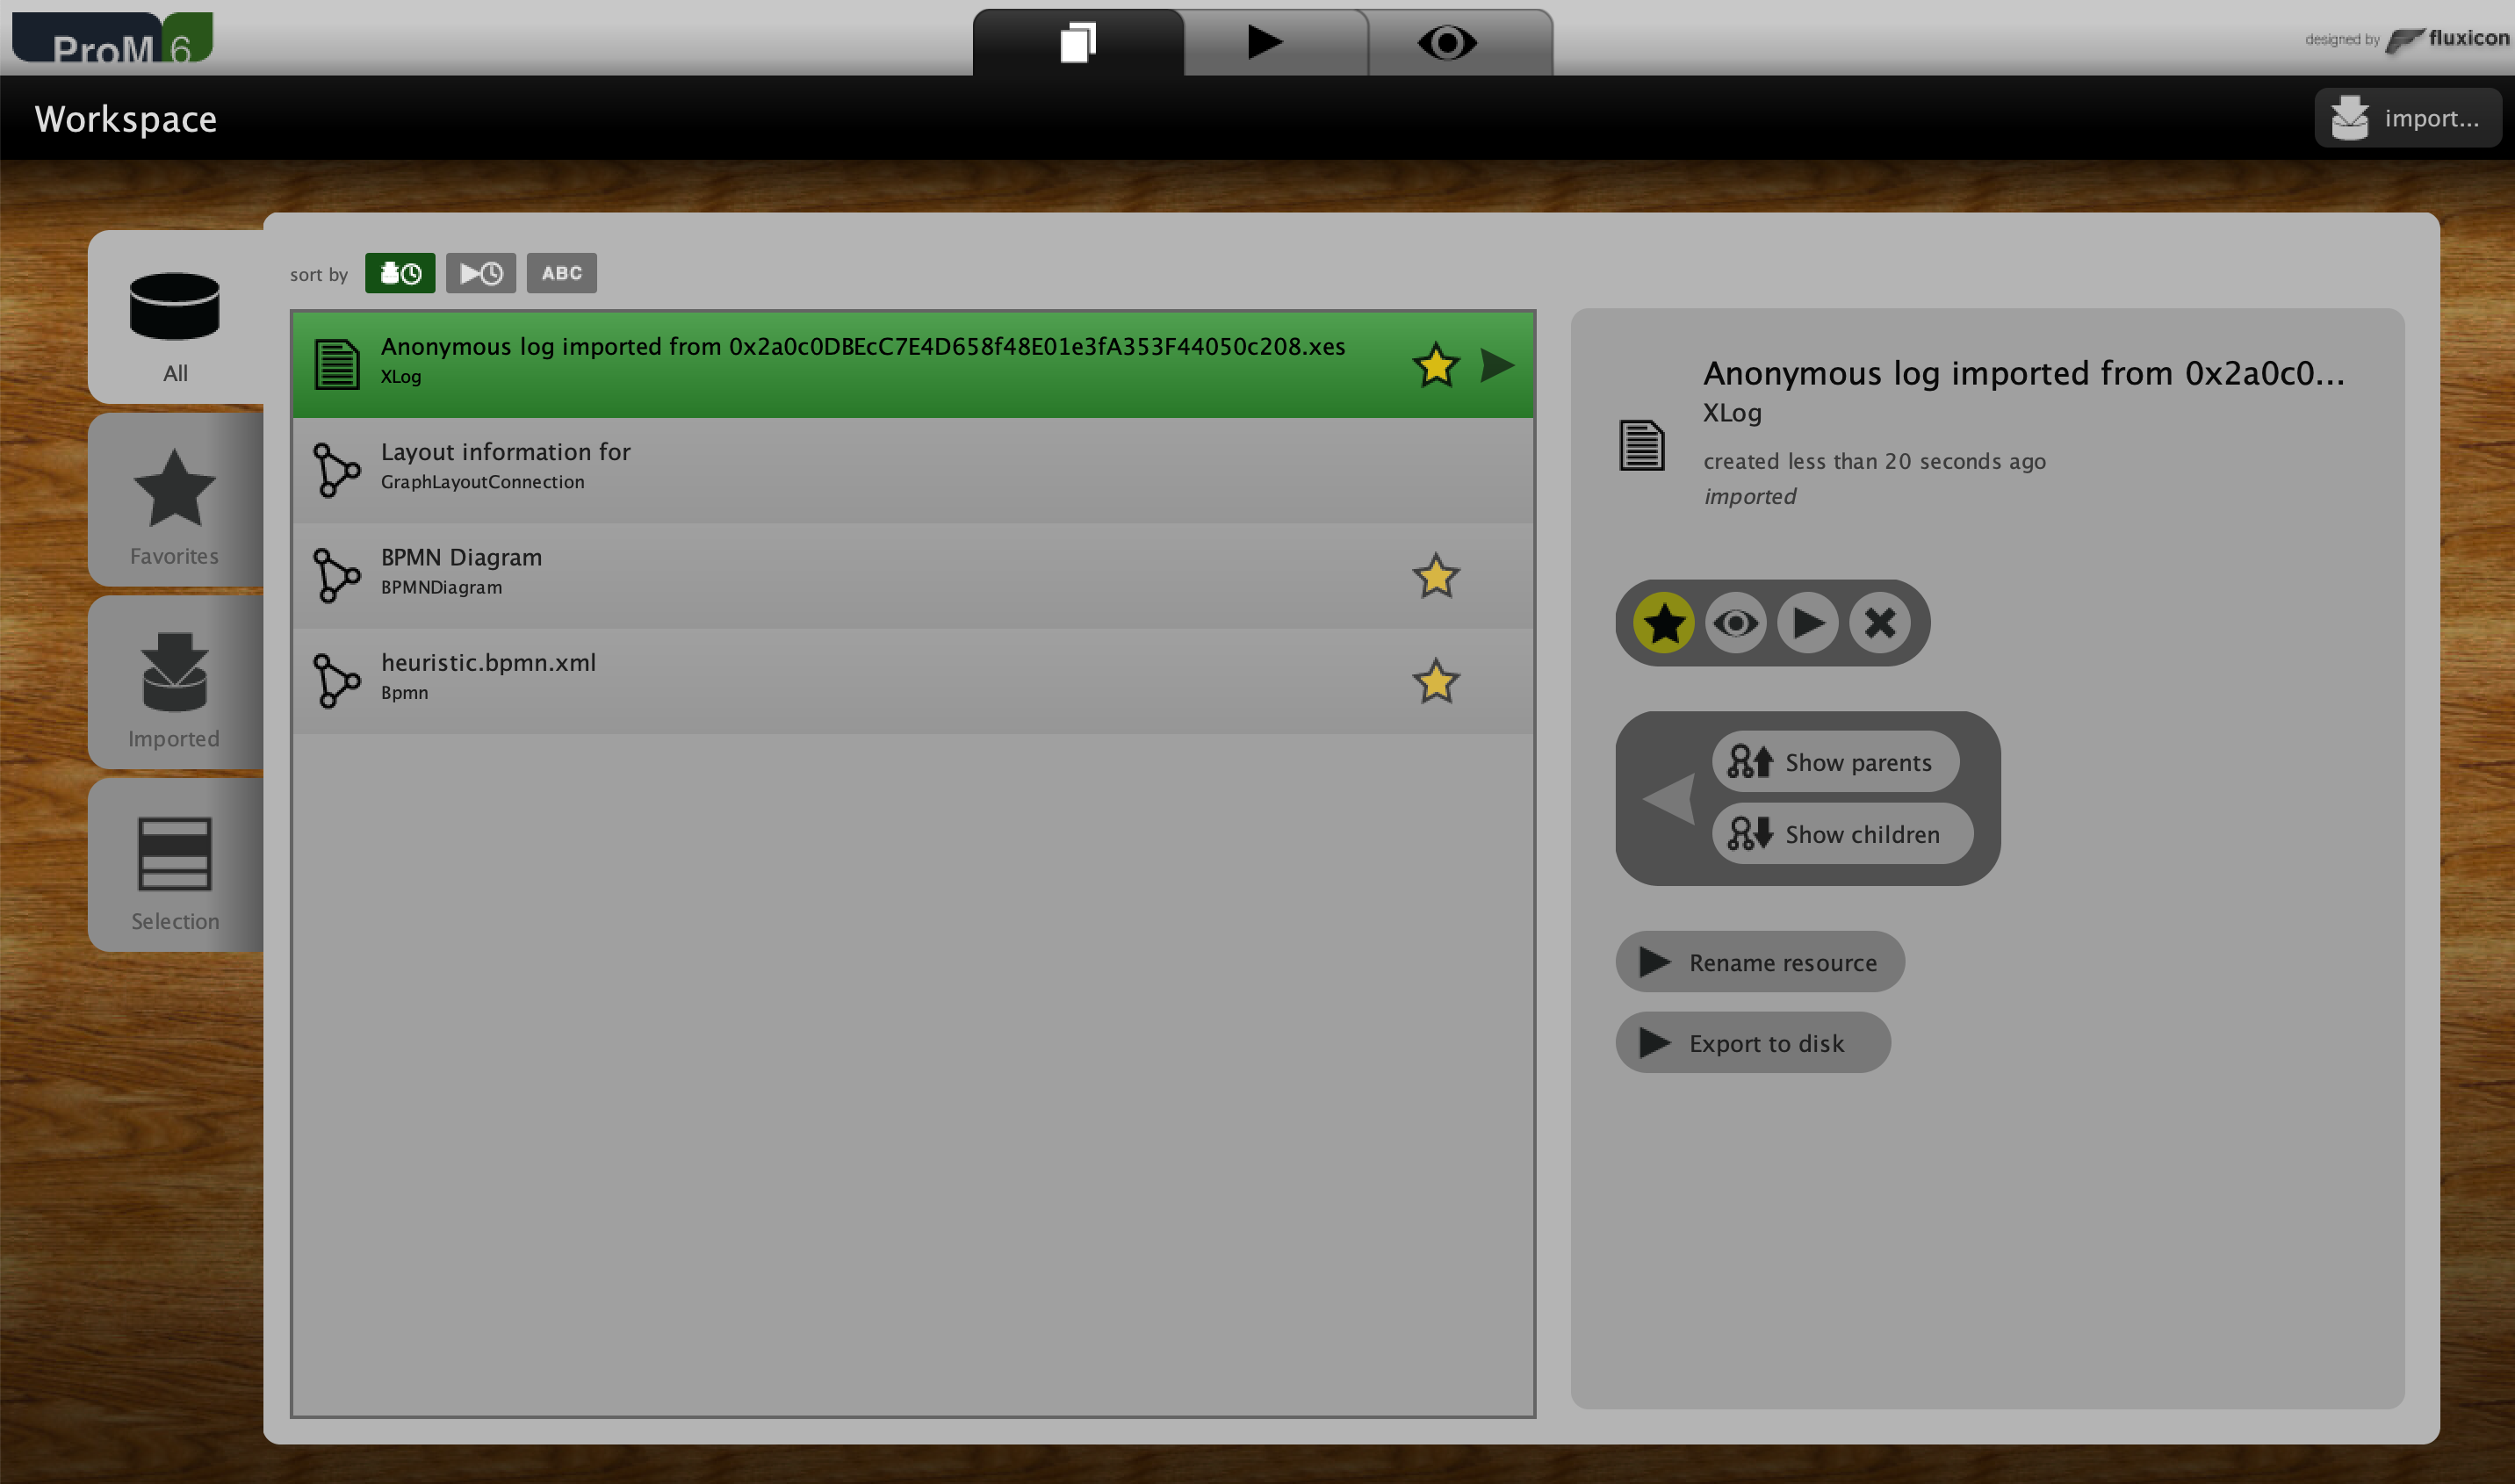
\includegraphics[width=\textwidth]{images/prom_screen_object.png}
    \caption{ProM object view screenshot}
    \label{images:prom_screen_object}
\end{figure}

In object view there are all objects you have work with: imported files, event logs, results of some ProM plugin, everything.
The visualization section renders objects in different ways: process trees, petri nets, images etc.

\begin{figure}[!ht]
    \centering
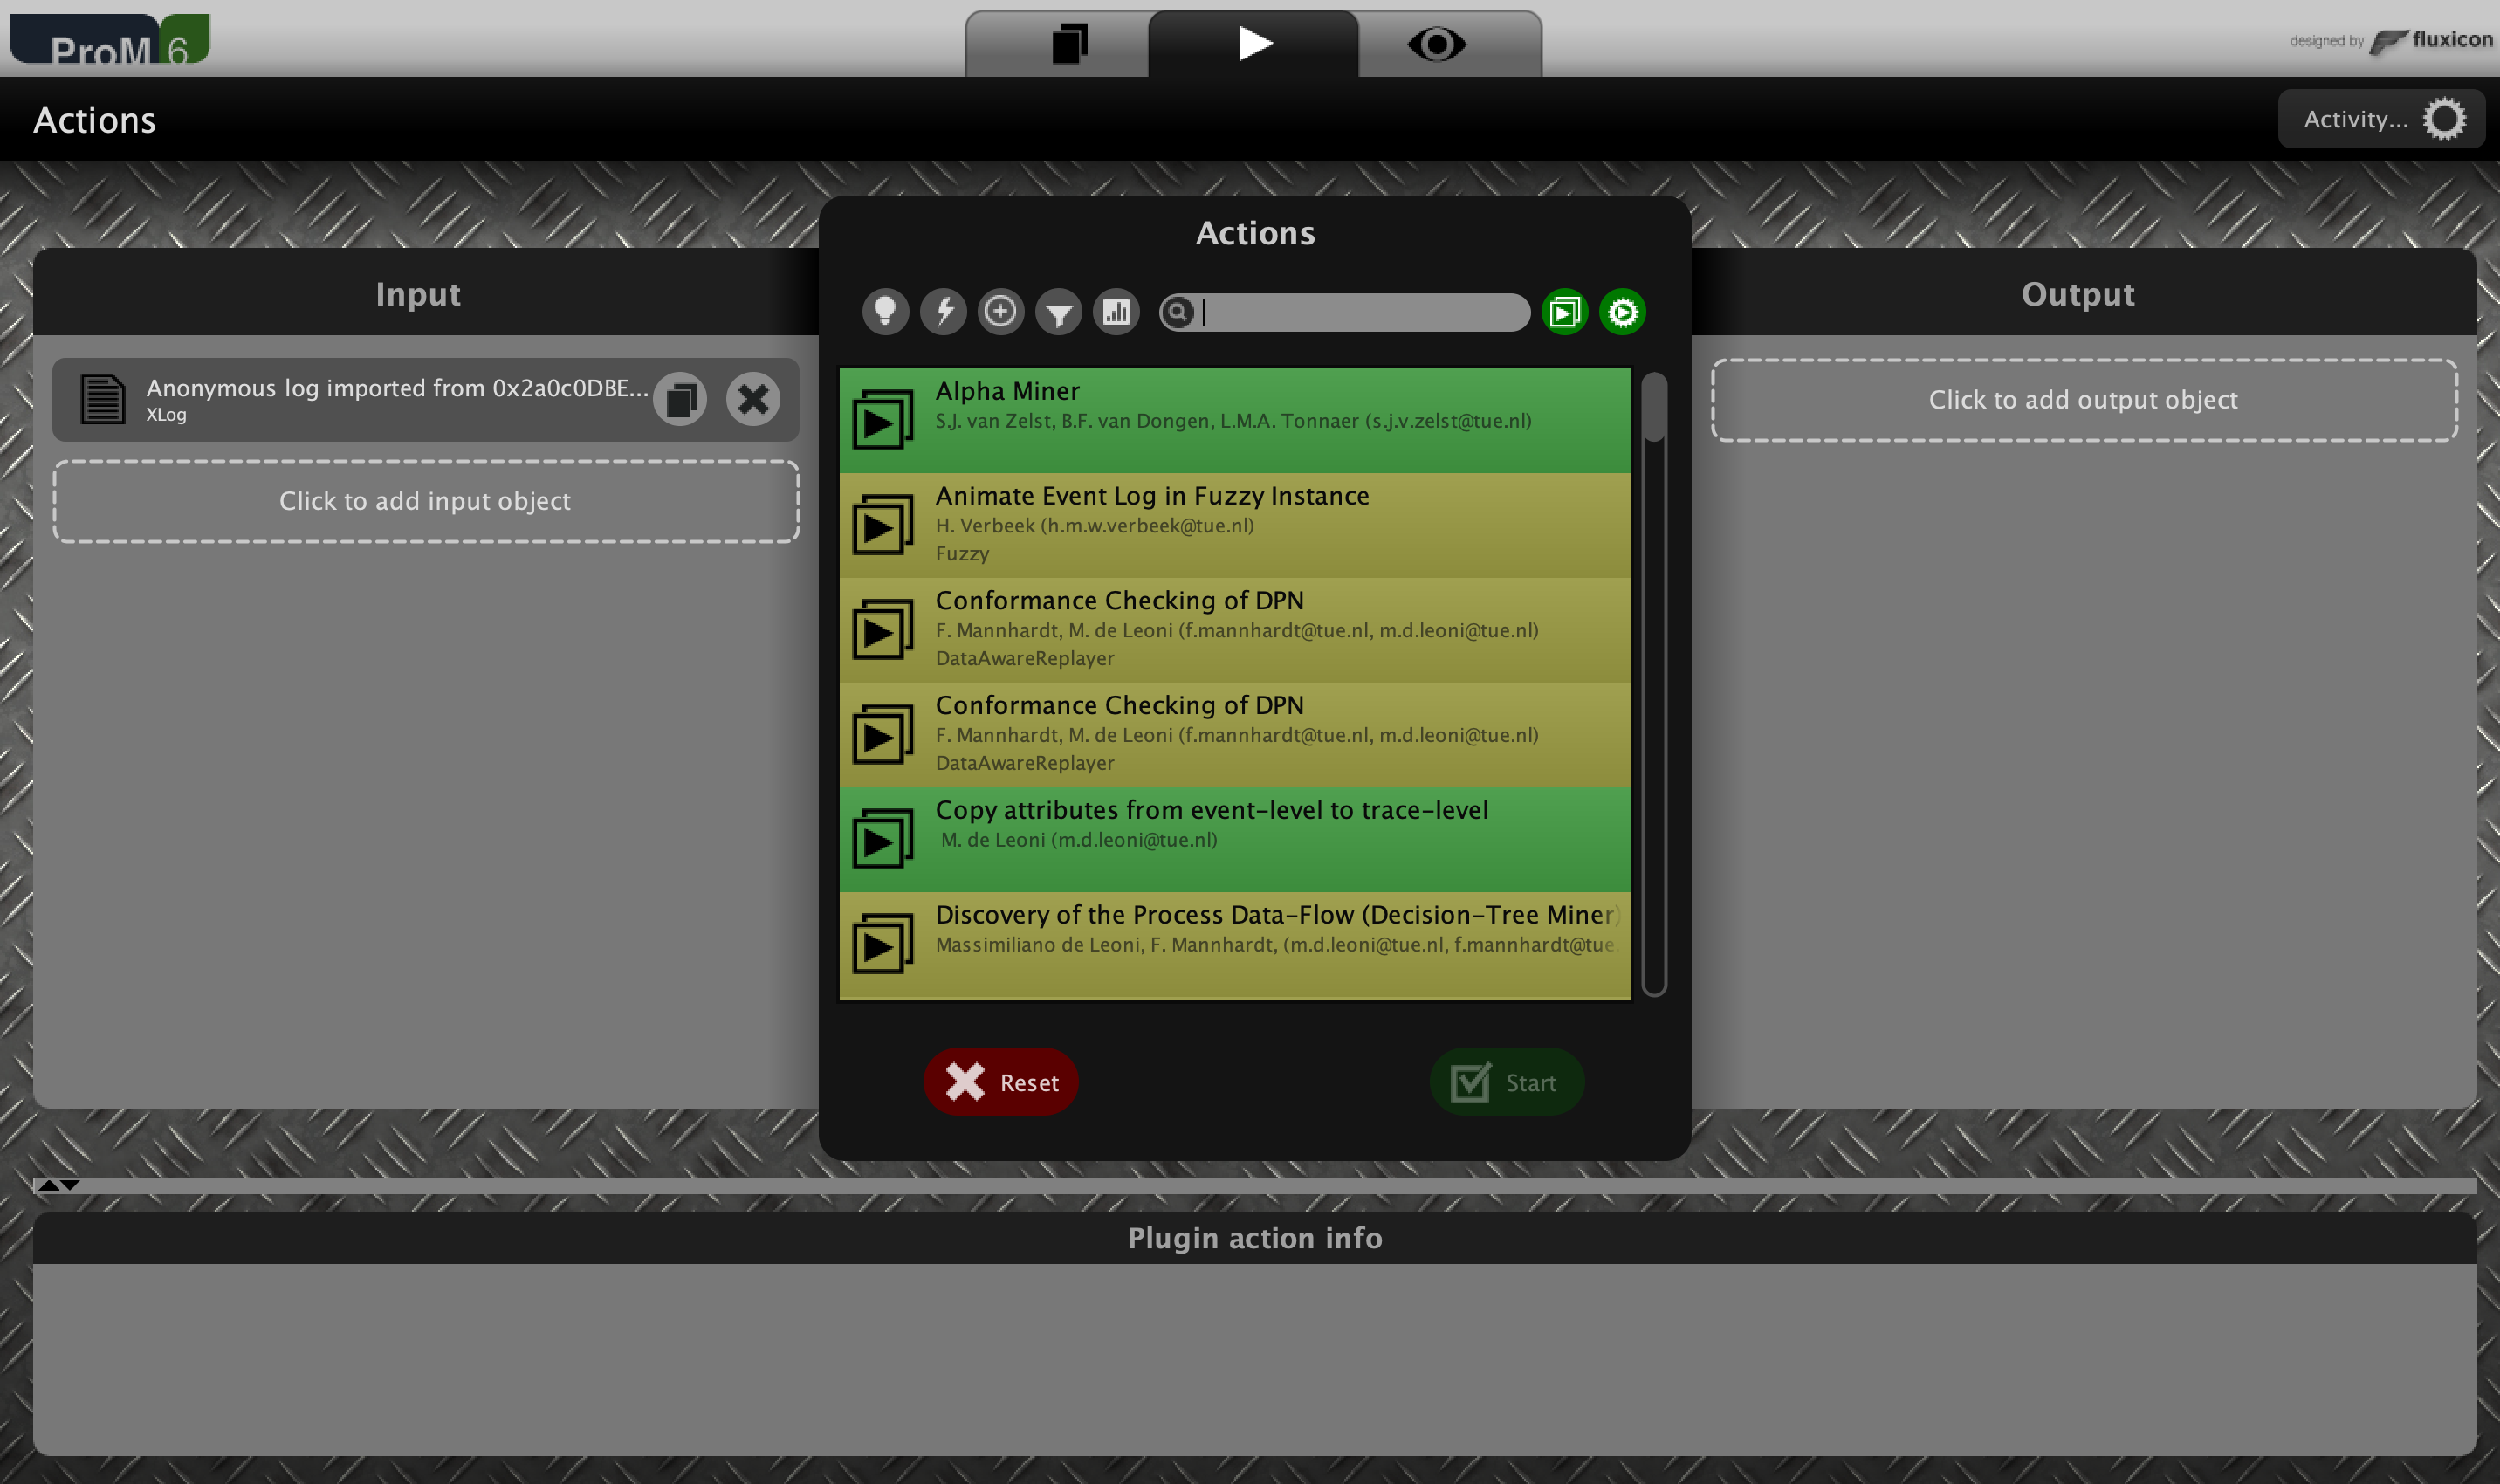
\includegraphics[width=\textwidth]{images/prom_screen_action.png}
    \caption{ProM action view screenshot}
    \label{images:prom_screen_action}
\end{figure}

The action view is the more interesting one: it is its own divided in other three subsections: input objects, feature to apply 
and output objects format/placeholder. In this section is possible to use all ProM techniques (discovery algorithms, 
conformance checking, etc.). The choise of the available actions is filtered based on selected inputs (for example chosen 
a xes file all discovery plugins are available to use but conformance checking cannot be done until the selection of a model to 
compare with log file).

The visualization section change its content based on the currente object selected: it can show a bpmn model, a petri net or 
some parameters measured with some plugin. Here is possible to export current showed data in the desired format.

In general ProM allows to import a lot of type of files (csv, xes, bpmn, etc.) and allow for exports too. It can be also 
used as a conversion tool.

ProM is also open source, this means that every one can write a plugin and make it public for who need it. Over that also its 
java libraries can be used in a custom application making available a powerful framework for developers.

ProM is a great tool, largely used and with a good community; the ui is enough simple to use. Its main disadvantage is its 
granularity: every plugin has a different structure even if their expected behaviour should be the same. In this case the 
great advantage to be an extensible framework became also its main disadvantages creating sometimes inconsistent behaviours 
between plugins.


\subsection{Apromore}
Apromore is an open-source business process analytics platform, supporting the full stack of process mining functionality, 
advanced features for authoring process models and managing process model collections. It is an online tool with different 
node around the world but there is also a desktop version. 

\begin{figure}[!ht]
    \centering
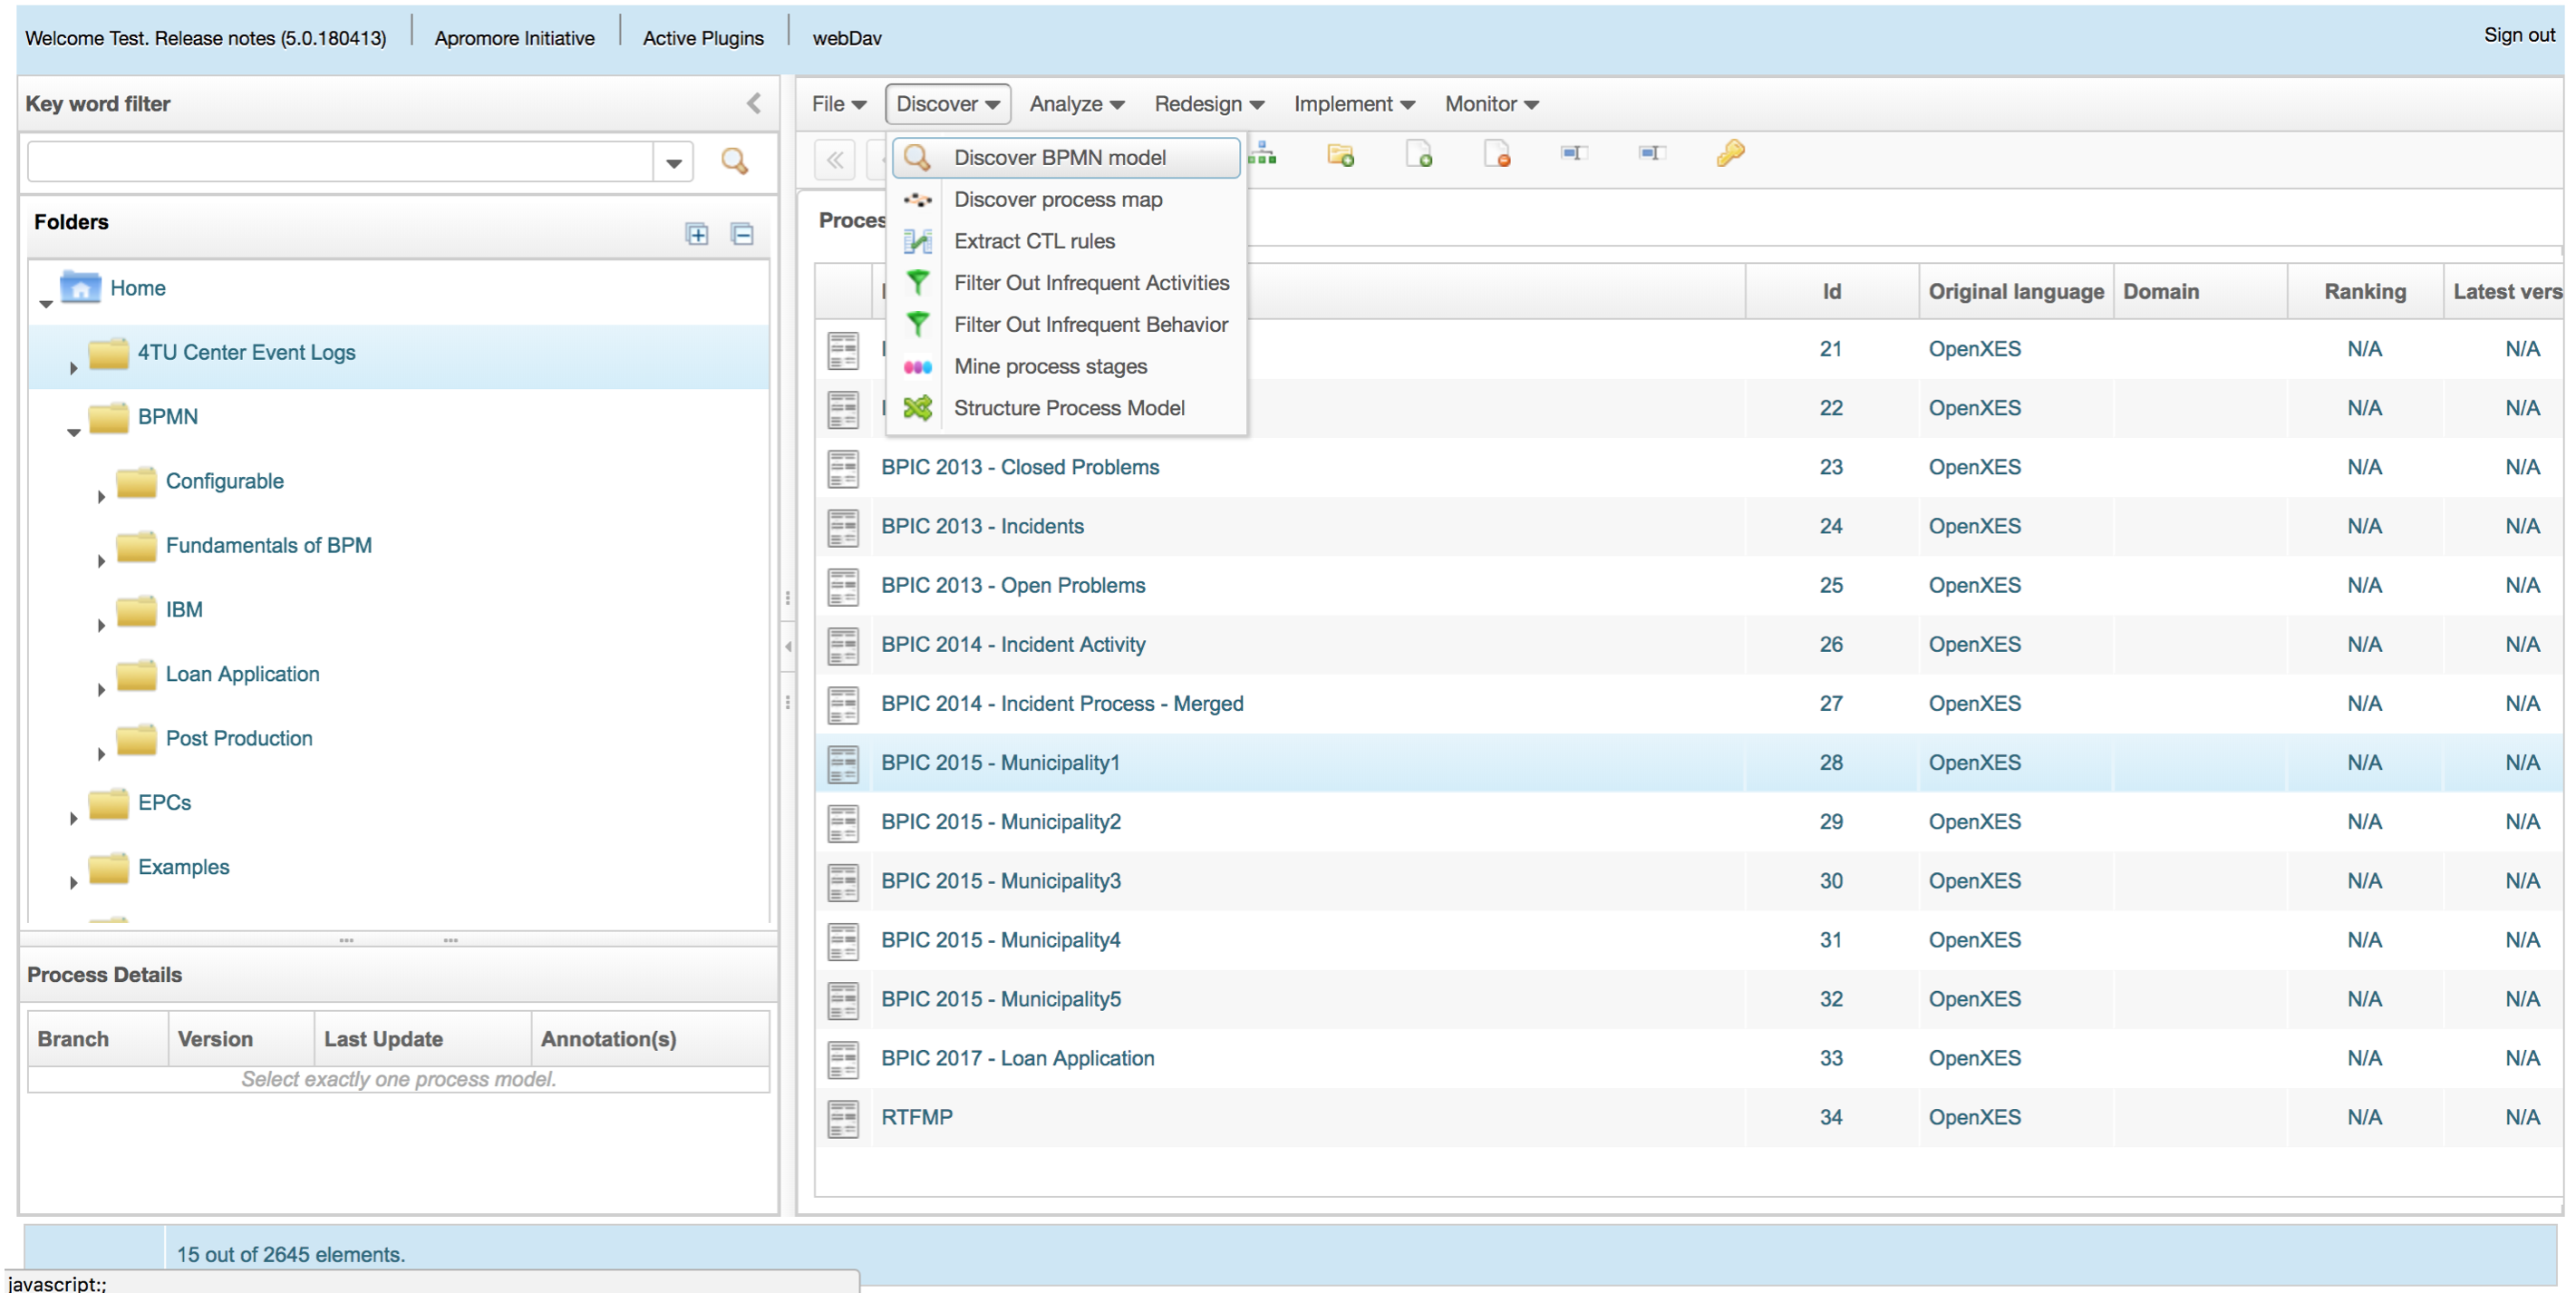
\includegraphics[width=\textwidth]{images/apromore_screen.png}
    \caption{Apromore main window}
    \label{images:apromore_screen}
\end{figure}

In Figure \ref{images:apromore_screen} the main Apromore window is displayed: at a first glance its UI is similar to a file 
server: on the left there is the directories hierarchy, at the center instead there are all files and subdirs of the current 
selected directory. On the top there is a toolbar with all the action that can be executed on the various objects. The 
process model editing commands are in a separate window that is also the visualization part of the tool.

This tool has a rich set of features for the managing of process models: it can be viewed as a process model repository with 
also great capabilities of editing of this models. In this case the set of algorithms supported is a bit different from ProM 
but with some commmon points. There are not a lot of features for quality checking but are supported a rich set of 
interesting capabilities:

\begin{itemize}
    \item animation of event log on top of BPMN models or process map
    \item conformance checking, where model's issues compared to the event log are highlighted
    \item filtering of infrequent activities or behaviors
    \item repair process model to align to event log
    \item train predictive models
\end{itemize}

As ProM even this tool supports all common standards (XES, BPMN, YAWL, etc.) and have a little set of plugins to extend 
the native available features (about 50). Even if this tool is extensible it is a bit less modular compared to ProM. Even in 
this case is possible to use its libraries in a custom project.

In general this is a tool with more features but a bit more complex to use compared to ProM.


\subsection{Disco}
Another tool avaiable in the market is Disco. It was developed by Fluxicon, as ProM, with special attention for user experience 
and speed. There is a basic free version and a complete licensed version. Disco has features for automated process discovery, 
process map animations, detailed statistics, exploration of processes down to single cases or events, filters, import/exports 
in all the main standard formats and in general for project management.

\begin{figure}[!ht]
    \centering
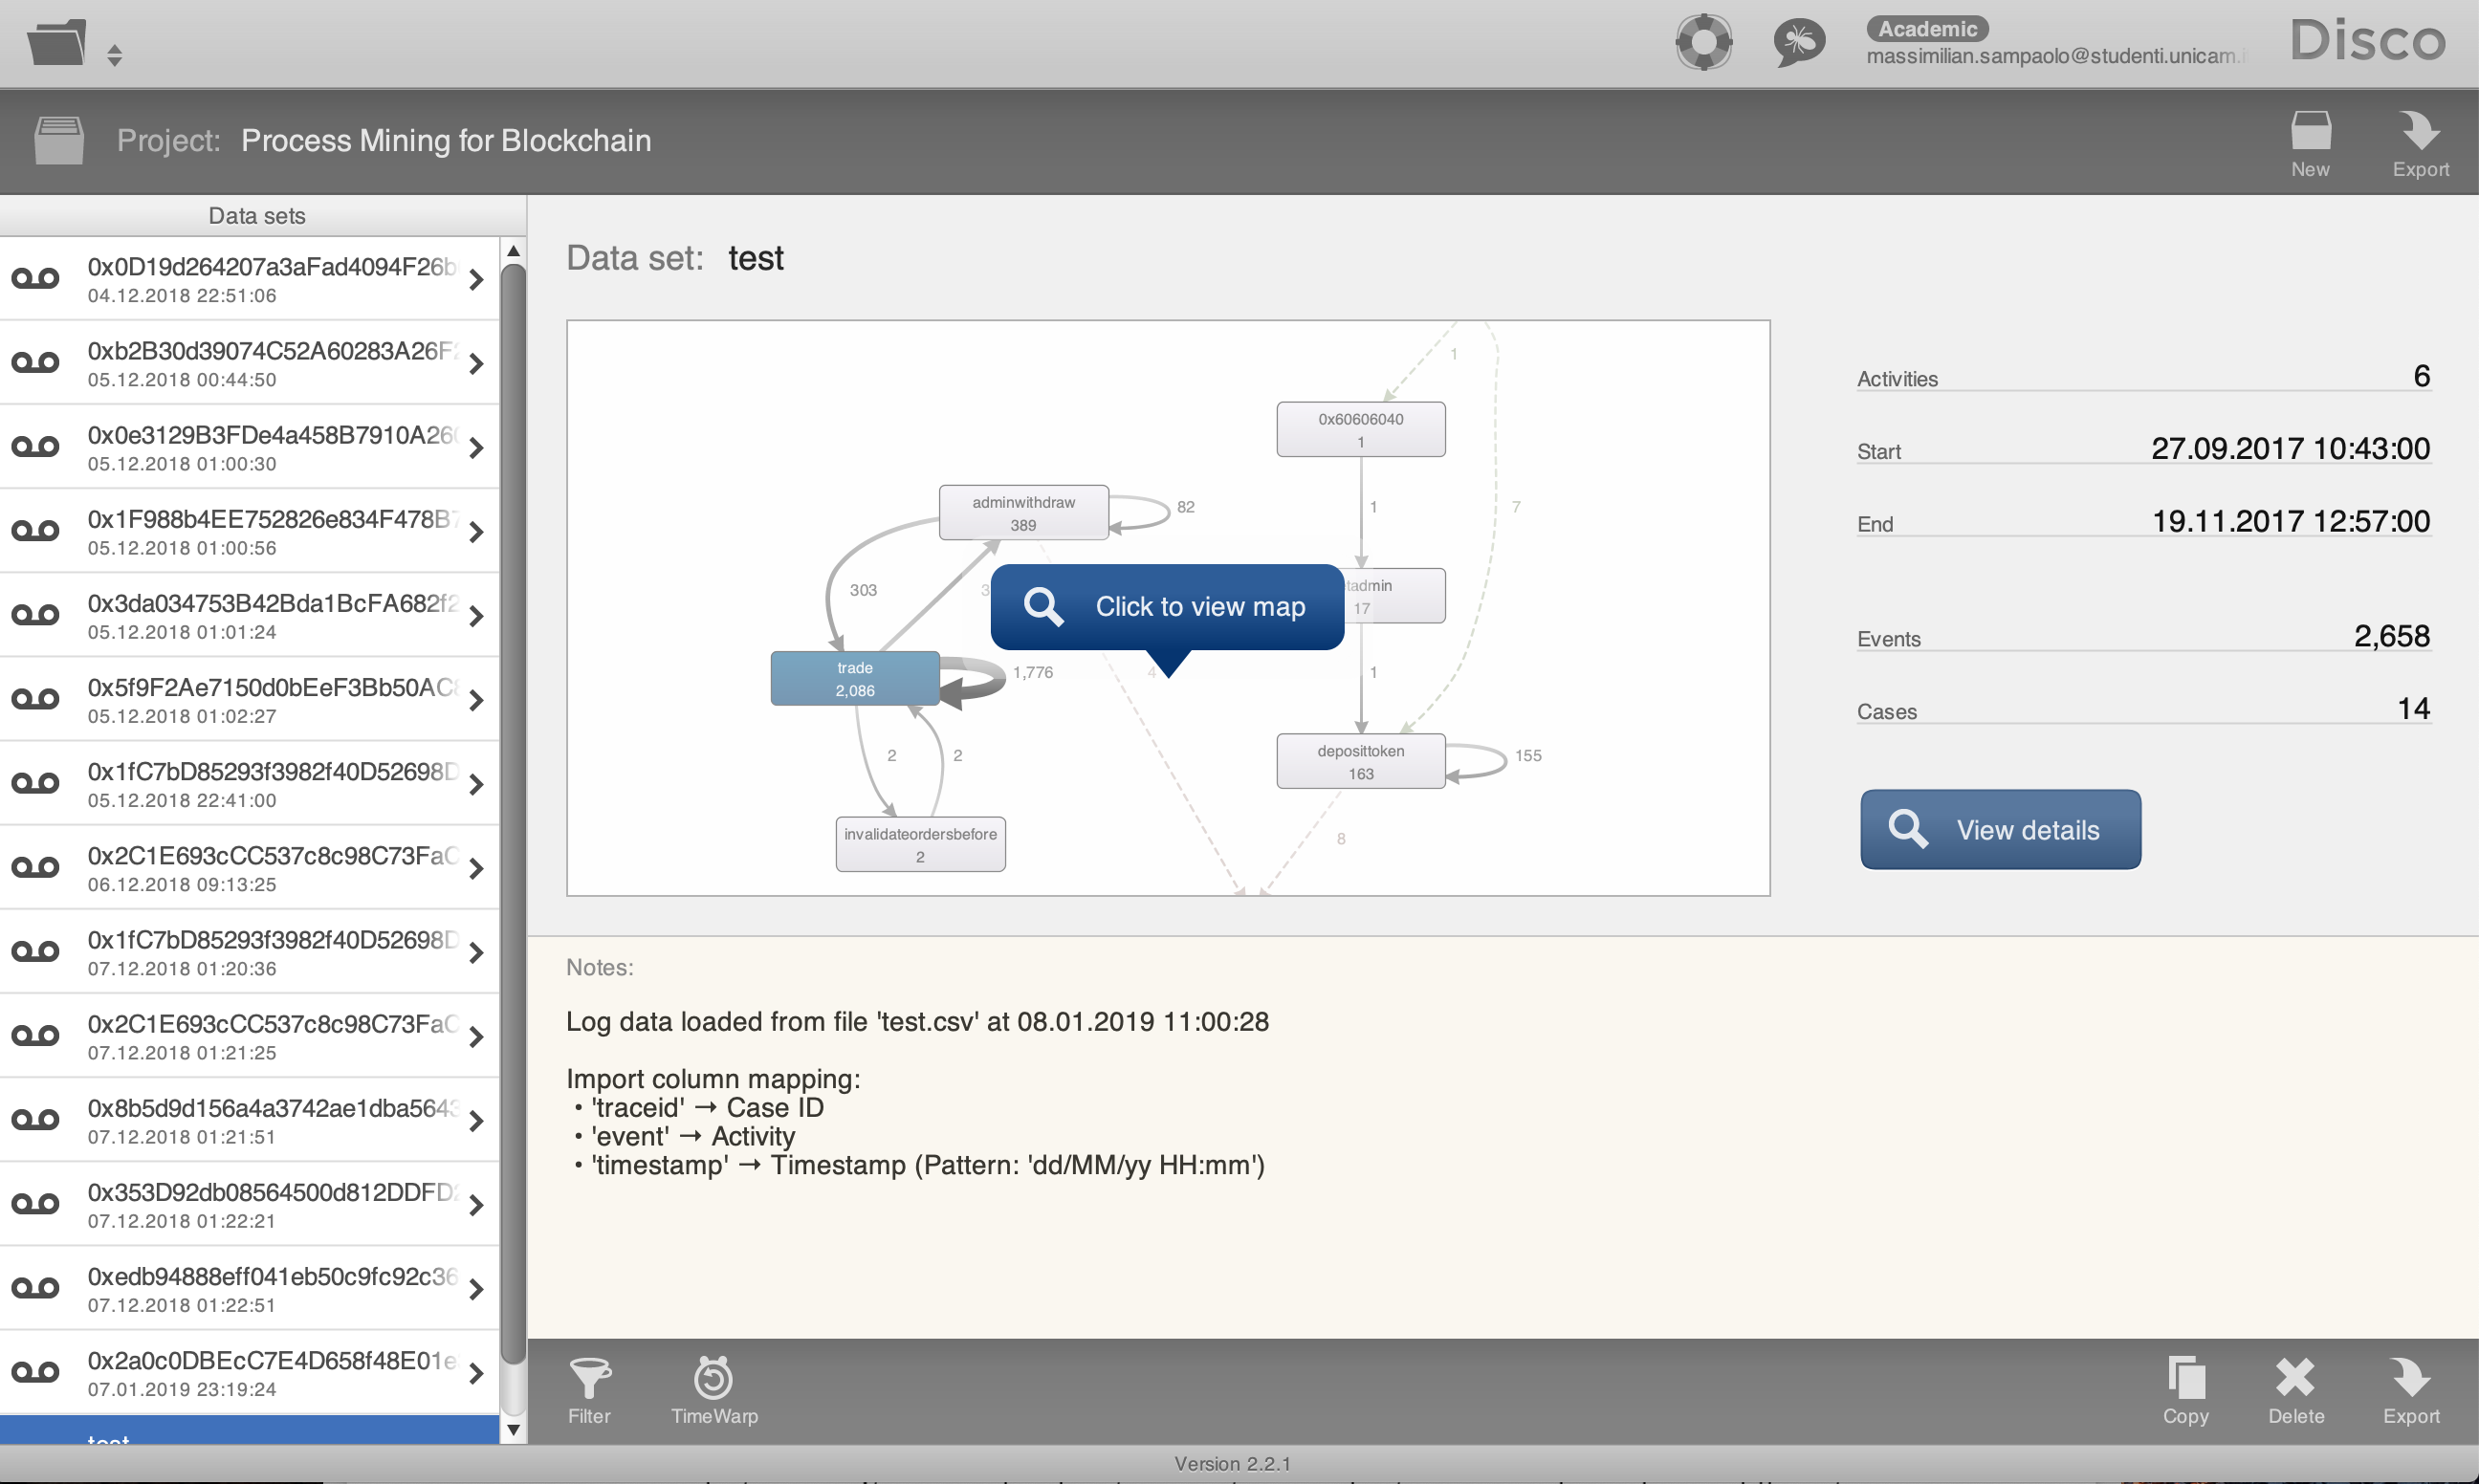
\includegraphics[width=\textwidth]{images/disco_screen.png}
    \caption{Disco main view}
    \label{images:disco_screen}
\end{figure}

In Figure \ref{images:disco_screen} there is a list of imported xes files on the left of the window, a detail of the current 
selection in the center of the window that contains the process map and some basic informations (the number of activities in 
the map, time interval in which the activities are included and the number of traces and events of the event log).

\begin{figure}[!ht]
    \centering
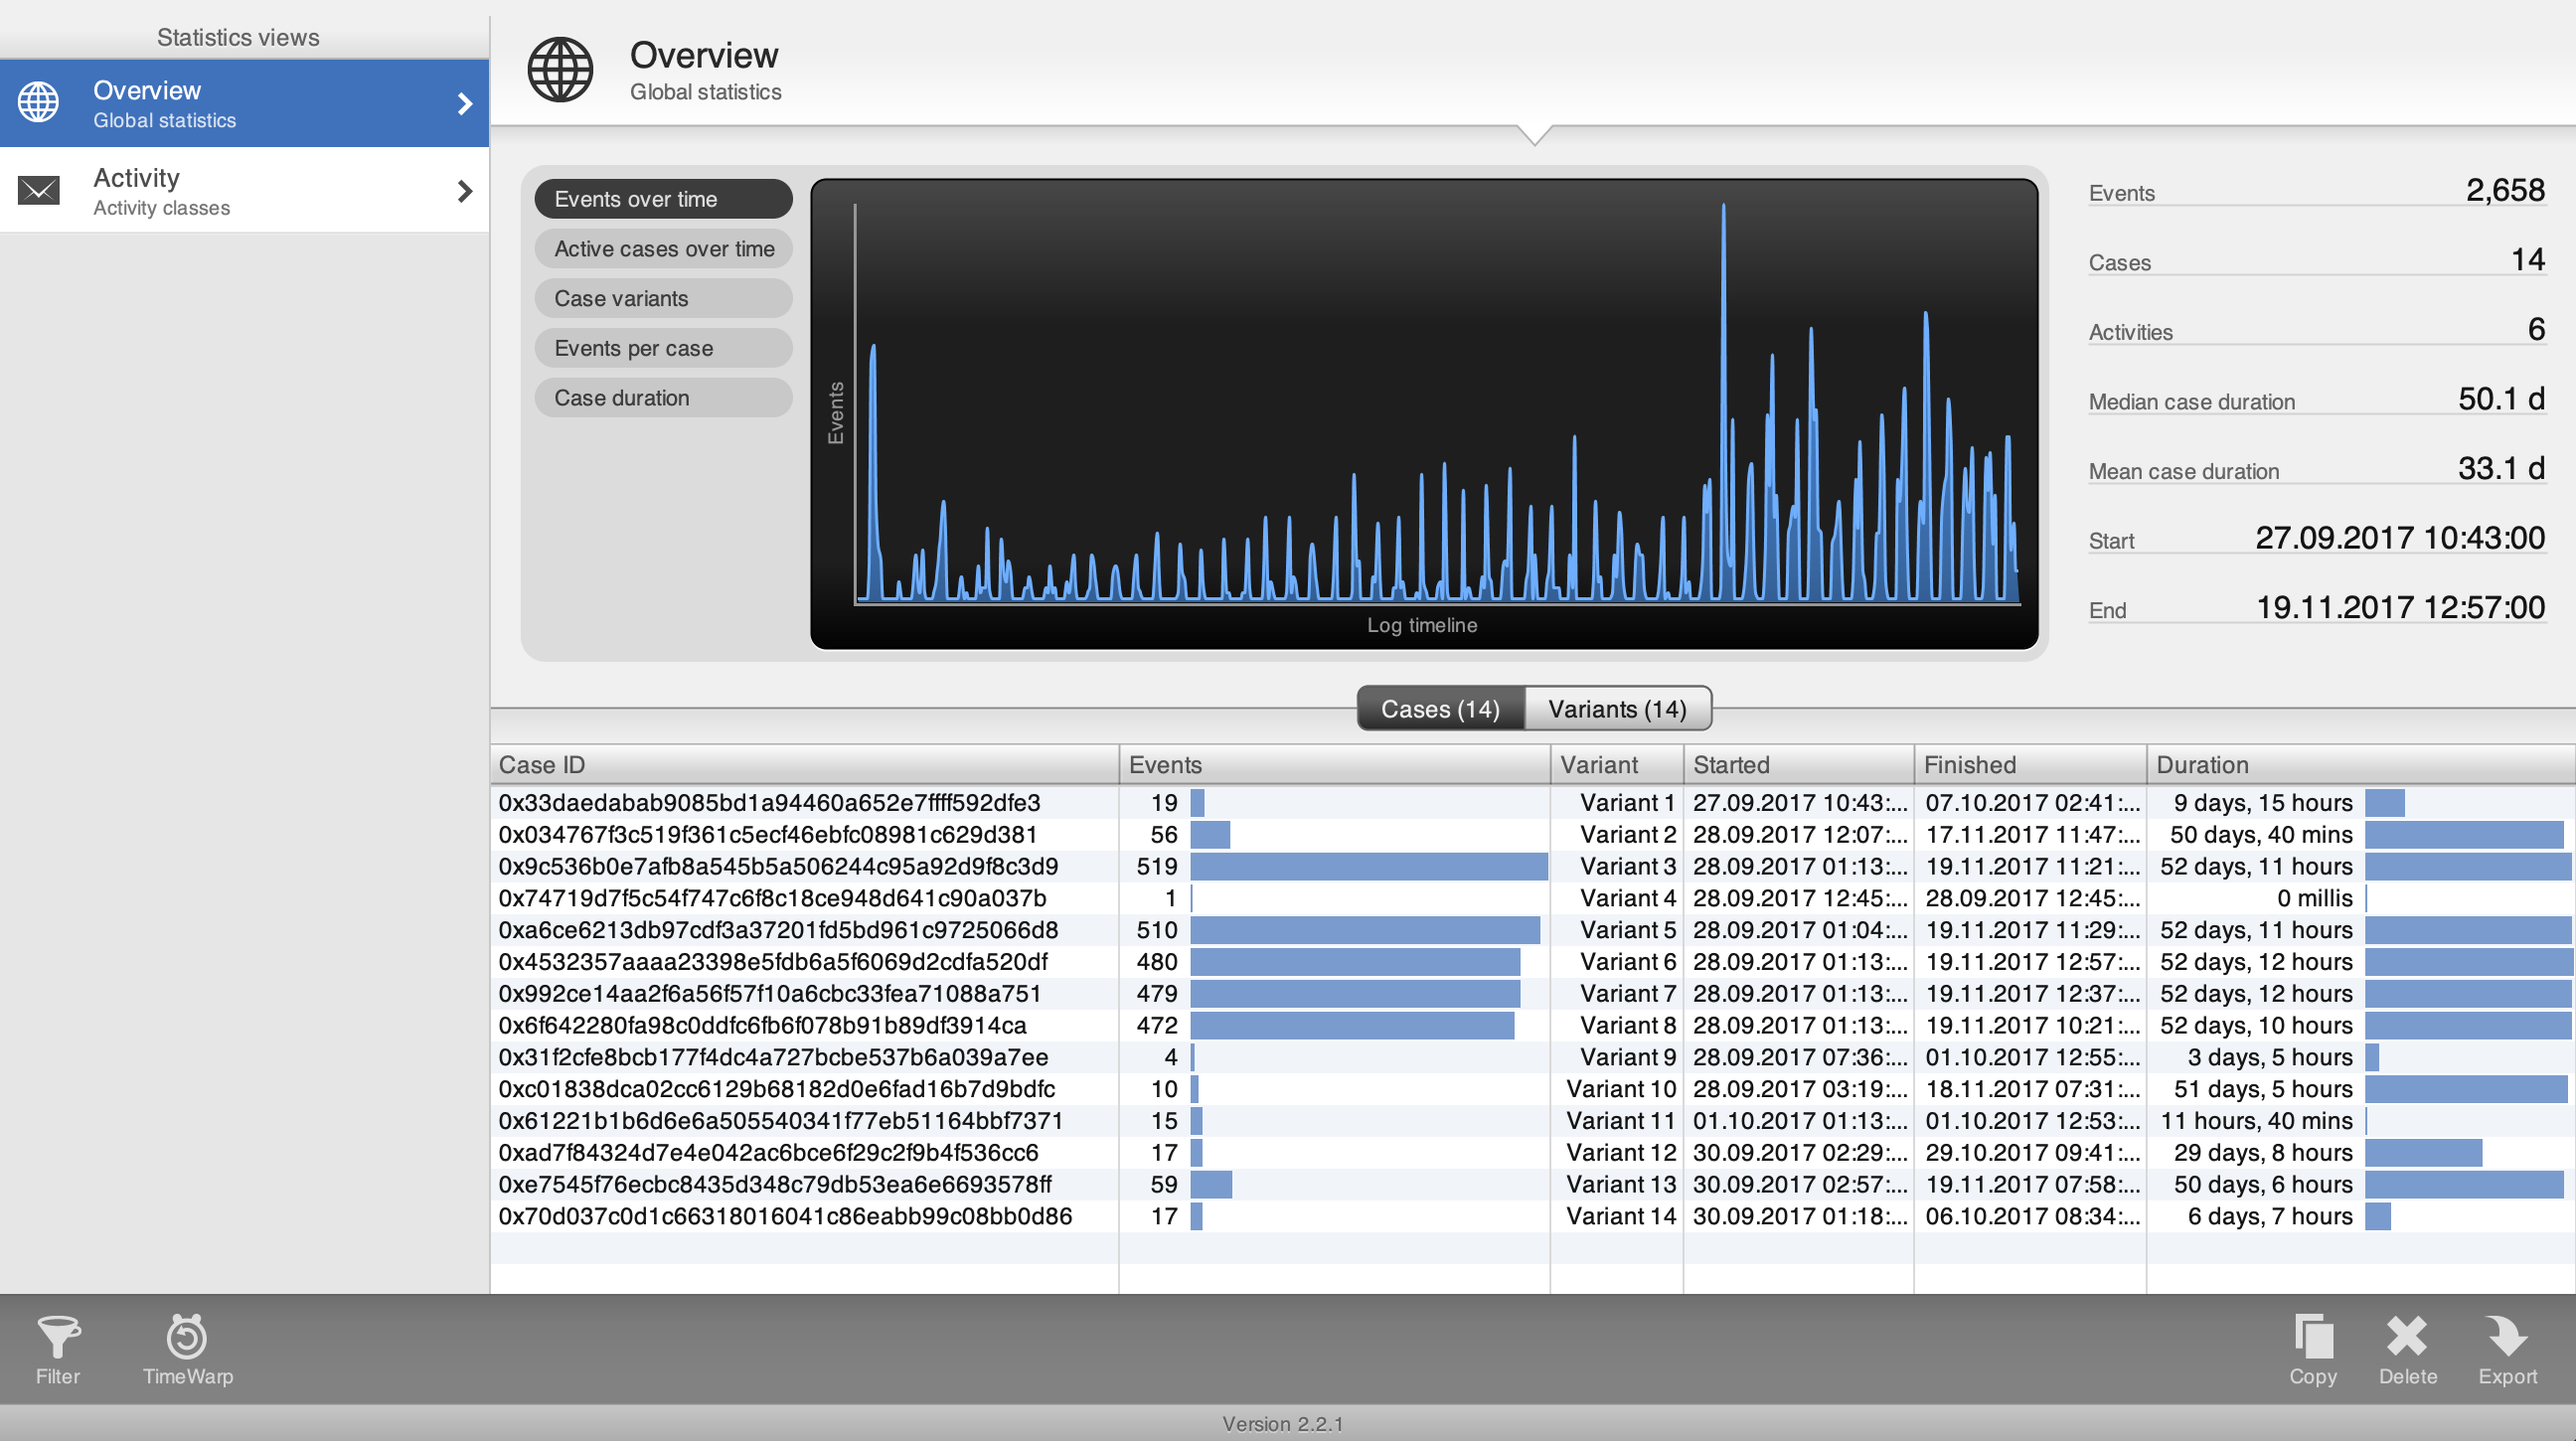
\includegraphics[width=\textwidth]{images/disco_screen_detail.png}
    \caption{Disco detail view}
    \label{images:disco_screen_detail}
\end{figure}

In Figure \ref{images:disco_screen_detail} are shown the details for a specific log/process map in disco: a lot of statistics 
are available with the permission to change the considered time interval. Also a deepening on one of the log event traces can be 
done.